% !TeX program = pdflatex -> bibtex -> pdflatex * 2
% Documento unificado. Compilar desde esta carpeta: pdflatex, biber propuesta, pdflatex, pdflatex.
% Si las bibliografias por curso muestran entradas de otro curso, borre propuesta.bbl (y propuesta.bcf) y vuelva a compilar todo el ciclo: un .bbl desactualizado respecto al .bcf desordena las refsections.
\documentclass[11pt]{report}

\input{propuesta-preamble}

\begin{document}

\input{propuesta-portada_departamento}
\tableofcontents


\clearpage

\chapter*{Introducción}
Este documento presenta un resumen de la Propuesta de Modificación Curricular que la Comisión de Malla Curricular ha desarrollado, con el apoyo de innumerables personas, para la transformación de la carrera de Matemática en la Universidad de Costa Rica. Contiene lo que la Comisión considera que son los elementos fundamentales para el análisis de la propuesta de parte de las personas del Departamento de Matemática. Se han omitido secciones relativas a contexto, estrategias pedagógicas, justificación, así como la descripción del proceso realizado a lo largo de estos años.

El documento completo se encuentra en desarrollo y podrá ser consultado para cuando se haga la propuesta completa en Asamblea de Escuela.

\chapter{Propósito de la carrera}
\chapter{Propósito de la carrera}


\chapter{Perfil de Egreso}


\section{Perfil de salida}

En la presente sección se presenta una síntesis del perfil de egreso elaborado en el periodo 2018–2020 por la Comisión de Malla Curricular de la carrera Bach. y Lic. en Matemática, como parte del proceso de transformación curricular que impulsa la Escuela de Matemática. El contenido completo del perfil aprobado se incluye en los anexos de este documento.

El perfil se ha adaptado para reflejar los cuatro grados incluidos esta nueva propuesta.

%\newpage 

\subsubsection{Bachillerato en matemática, énfasis en matemática pura}


\begin{table}[H]
\centering
\renewcommand{\arraystretch}{1.3}
\begin{tabular}{|c|p{9cm}|}
\hline
\cellcolor[HTML]{00C0F3}\textbf{Código(s)} & \cellcolor[HTML]{00C0F3}\textbf{Enunciado de la dimensión declarativa} \\
\hline
CDP01 & Conoce y comprende los fundamentos matemáticos —incluyendo la lógica, la teoría de números y la geometría euclídea— y los principios formales que sustentan el razonamiento y la argumentación rigurosa. \\
\hline
CDP02 & Conoce el uso de software especializado, los fundamentos de la programación y la computación científica, así como las técnicas básicas de análisis numérico para formular, explorar y resolver problemas matemáticos mediante enfoques computacionales. \\
\hline
CDP03 & Conoce los conceptos, métodos y aplicaciones básicos del cálculo y del álgebra lineal como fundamentos de la formación matemática. \\
\hline
CDP04 & Conoce los conceptos y técnicas de las ecuaciones diferenciales, la teoría de la medida, la probabilidad y los procesos estocásticos, así como del análisis complejo y funcional. \\
\hline
CDP05 & Conoce los fundamentos y resultados básicos de la geometría y la topología. \\
\hline
CDP06 & Conoce las estructuras y resultados fundamentales del álgebra abstracta. 
\\
\hline
CDP07 & Conoce las estructuras y resultados fundamentales de algún área de especialización en matemática pura más allá de las antes expuestas. 
\\
\hline
\end{tabular}
\caption{Tabla de conocimientos declarativos o saber conocer.}
\label{tab:declarativa-egreso-integrada}
\end{table}

%\newpage

\begin{table}[H]
\centering
\renewcommand{\arraystretch}{1.3}
\begin{tabular}{|c|p{9cm}|}
\hline
\cellcolor[HTML]{00C0F3}\textbf{Código(s)}  & \cellcolor[HTML]{00C0F3}\textbf{Enunciado de la dimensión procedimental} \\
\hline
CP01 & Aplica pensamiento operacional, abstracto y formal para analizar, resolver y sintetizar problemas matemáticos. \\
\hline
CP02 & Formula conjeturas, resuelve problemas, interpreta resultados y se comunica de manera coherente en lenguaje matemático formal. \\
\hline
CP03 & Utiliza tecnologías y software científico para explorar, validar y resolver problemas matemáticos.\\
\hline
CP04 & Participa activamente en discusiones científicas y divulga el conocimiento matemático de forma accesible a diferentes audiencias.\\
\hline
\end{tabular}
\caption{Tabla de conocimientos procedimentales o saber hacer.}
\label{tab:procedimental-egreso-integrada}
\end{table}

\begin{table}[H]
\centering
\renewcommand{\arraystretch}{1.3}
\begin{tabular}{|c|p{9cm}|}
\hline
\cellcolor[HTML]{00C0F3}\textbf{Código(s)} & \cellcolor[HTML]{00C0F3}\textbf{Enunciado de la dimensión actitudinal} \\
\hline
CA01 & Manifiesta respeto por la diversidad humana, matemática, científica y cultural, fomentando un ambiente inclusivo y de valoración mutua. \\
\hline
CA02 & Se comunica con claridad, colabora en equipos académicos y profesionales, y mantiene una disposición al autoaprendizaje y al liderazgo.\\
\hline
CA03 & Demuestra conciencia social y participación ciudadana, con una visión sociocultural e integral de la sociedad en la que la ciencia y la matemática ocupan un lugar relevante.\\
\hline
CA04 & Ejerce pensamiento crítico, actúa con integridad ética y evalúa con rigor las prácticas científicas y académicas.\\
\hline
CA05 & Utiliza su conocimiento matemático para resolver problemas académicos y profesionales, adaptándolo a distintos contextos y necesidades.\\
\hline
CA06 & Mantiene un interés permanente por los desarrollos de la investigación científica y matemática, valorando la actualización como parte de su formación profesional.\\
\hline
\end{tabular}
\caption{Tabla de conocimientos actitudinales, o saber ser.}
\label{tab:actitudinal-egreso-integrada}
\end{table}


\subsubsection{Bachillerato en matemática, énfasis en matemática aplicada}



\begin{table}[H]
\centering
\renewcommand{\arraystretch}{1.3}
\begin{tabular}{|c|p{9cm}|}
\hline
\cellcolor[HTML]{00C0F3}\textbf{Código(s)} & \cellcolor[HTML]{00C0F3}\textbf{Enunciado de la dimensión declarativa} \\
\hline
CDA01 & Conoce y comprende los fundamentos matemáticos —incluyendo la lógica, la teoría de números y la geometría euclídea— y los principios formales que sustentan el razonamiento y la argumentación rigurosa. \\
\hline
CDA02 & Conoce el uso de software especializado, los fundamentos de la programación y la computación científica, así como las técnicas básicas de análisis numérico para formular, explorar y resolver problemas matemáticos mediante enfoques computacionales. \\
\hline
CDA03 & Conoce los conceptos, métodos y aplicaciones básicos del cálculo y del álgebra lineal como fundamentos de la formación matemática. \\
\hline
CDA04 & Conoce los conceptos y técnicas de las ecuaciones diferenciales, la teoría de la medida, la probabilidad y los procesos estocásticos, así como del análisis complejo y funcional. \\
\hline
CDA05 & Conoce los principios de la matemática aplicada, por ejemplo por medio de la modelación, la estadística o el análisis de datos, para resolver problemas y tomar decisiones en ámbitos como la industria, la banca y otros sectores.
\\
\hline
CDA06 & Conoce las principales tecnologías de aplicación de la matemática, por ejemplo ejemplo la programación y computación científica para aplicar conceptos teóricos a problemas reales.
\\
\hline
CDA07 & Conoce las estructuras y resultados fundamentales de algún área de especialización en matemática aplicada más allá de las antes expuestas. 
\\
\hline
\end{tabular}
\caption{Tabla de conocimientos declarativos o saber conocer.}
\label{tab:declarativa-egreso-integrada}
\end{table}

%\newpage

\begin{table}[H]
\centering
\renewcommand{\arraystretch}{1.3}
\begin{tabular}{|c|p{9cm}|}
\hline
\cellcolor[HTML]{00C0F3}\textbf{Código(s)}  & \cellcolor[HTML]{00C0F3}\textbf{Enunciado de la dimensión procedimental} \\
\hline
CP01 & Aplica pensamiento operacional, abstracto y formal para analizar, resolver y sintetizar problemas matemáticos. \\
\hline
CP02 & Formula conjeturas, resuelve problemas, interpreta resultados y se comunica de manera coherente en lenguaje matemático formal. \\
\hline
CP03 & Utiliza tecnologías y software científico para explorar, validar y resolver problemas matemáticos.\\
\hline
CP04 & Participa activamente en discusiones científicas y divulga el conocimiento matemático de forma accesible a diferentes audiencias.\\
\hline
\end{tabular}
\caption{Tabla de conocimientos procedimentales o saber hacer.}
\label{tab:procedimental-egreso-integrada}
\end{table}


%\newpage

\begin{table}[H]
\centering
\renewcommand{\arraystretch}{1.3}
\begin{tabular}{|c|p{9cm}|}
\hline
\cellcolor[HTML]{00C0F3}\textbf{Código(s)} & \cellcolor[HTML]{00C0F3}\textbf{Enunciado de la dimensión actitudinal} \\
\hline
CA01 & Manifiesta respeto por la diversidad humana, matemática, científica y cultural, fomentando un ambiente inclusivo y de valoración mutua. \\
\hline
CA02 & Se comunica con claridad, colabora en equipos académicos y profesionales, y mantiene una disposición al autoaprendizaje y al liderazgo.\\
\hline
CA03 & Demuestra conciencia social y participación ciudadana, con una visión sociocultural e integral de la sociedad en la que la ciencia y la matemática ocupan un lugar relevante.\\
\hline
CA04 & Ejerce pensamiento crítico, actúa con integridad ética y evalúa con rigor las prácticas científicas y académicas.\\
\hline
CA05 & Utiliza su conocimiento matemático para resolver problemas académicos y profesionales, adaptándolo a distintos contextos y necesidades.\\
\hline
CA06 & Mantiene un interés permanente por los desarrollos de la investigación científica y matemática, valorando la actualización como parte de su formación profesional.\\
\hline
\end{tabular}
\caption{Tabla de conocimientos actitudinales o saber ser.}
\label{tab:actitudinal-egreso-integrada}
\end{table}


\subsubsection{Licenciatura en matemática, énfasis en matemática pura}


En adición a los conocimientos enunciados para el bachillerato, con la licenciatura se tendrían los siguientes.

\begin{table}[H]
\centering
\renewcommand{\arraystretch}{1.3}
\begin{tabular}{|c|p{9cm}|}
\hline
\cellcolor[HTML]{00C0F3}\textbf{Código(s)} & \cellcolor[HTML]{00C0F3}\textbf{Enunciado de la dimensión declarativa} \\
\hline
CDA08 & Conoce estructuras y resultados de nivel intermedio para algunas áreas medulares de especialización en matemática pura. 
\\
\hline
\end{tabular}
\caption{Tabla de conocimientos declarativos o saber conocer.}
\label{tab:declarativa-egreso-integrada}
\end{table}

%\newpage

\begin{table}[H]
\centering
\renewcommand{\arraystretch}{1.3}
\begin{tabular}{|c|p{9cm}|}
\hline
\cellcolor[HTML]{00C0F3}\textbf{Código(s)}  & \cellcolor[HTML]{00C0F3}\textbf{Enunciado de la dimensión procedimental} \\
\hline
CP05 & Aplica pensamiento operacional, abstracto y formal, con fuentes transversales de varias áreas, para formular, analizar y resolver problemas matemáticos. \\
\hline
\end{tabular}
\caption{Tabla de conocimientos procedimentales o saber hacer.}
\label{tab:procedimental-egreso-integrada}
\end{table}


\begin{table}[H]
\centering
\renewcommand{\arraystretch}{1.3}
\begin{tabular}{|c|p{9cm}|}
\hline
\cellcolor[HTML]{00C0F3}\textbf{Código(s)} & \cellcolor[HTML]{00C0F3}\textbf{Enunciado de la dimensión actitudinal} \\
\hline
CA06 & Muestra iniciativa y autonomía para formular preguntas, explorar problemas matemáticos y profundizar en ellos más allá de los procedimientos conocidos.\\
\hline
\end{tabular}
\caption{Tabla de conocimientos actitudinales o saber ser.}
\label{tab:actitudinal-egreso-integrada}
\end{table}

\subsubsection{Licenciatura en matemática, énfasis en matemática aplicada}

En adición a los conocimientos enunciados para el bachillerato, con la licenciatura se tendrían los siguientes.

\begin{table}[H]
\centering
\renewcommand{\arraystretch}{1.3}
\begin{tabular}{|c|p{9cm}|}
\hline
\cellcolor[HTML]{00C0F3}\textbf{Código(s)} & \cellcolor[HTML]{00C0F3}\textbf{Enunciado de la dimensión declarativa} \\
\hline
CDA08 & Conoce estructuras y resultados de nivel intermedio para algunas áreas medulares de especialización en matemática aplicada. 
\\
\hline
\end{tabular}
\caption{Tabla de conocimientos declarativos o saber conocer.}
\label{tab:declarativa-egreso-integrada}
\end{table}

%\newpage

\begin{table}[H]
\centering
\renewcommand{\arraystretch}{1.3}
\begin{tabular}{|c|p{9cm}|}
\hline
\cellcolor[HTML]{00C0F3}\textbf{Código(s)}  & \cellcolor[HTML]{00C0F3}\textbf{Enunciado de la dimensión procedimental} \\
\hline
CP05 & Aplica pensamiento operacional, abstracto y formal, con fuentes transversales de varias áreas, para formular, analizar y resolver problemas matemáticos. \\
\hline
\end{tabular}
\caption{Tabla de conocimientos procedimentales o saber hacer.}
\label{tab:procedimental-egreso-integrada}
\end{table}


\begin{table}[H]
\centering
\renewcommand{\arraystretch}{1.3}
\begin{tabular}{|c|p{9cm}|}
\hline
\cellcolor[HTML]{00C0F3}\textbf{Código(s)} & \cellcolor[HTML]{00C0F3}\textbf{Enunciado de la dimensión actitudinal} \\
\hline
CA06 & Muestra iniciativa y autonomía para formular preguntas, explorar problemas matemáticos y profundizar en ellos más allá de los procedimientos conocidos.\\
\hline
\end{tabular}
\caption{Tabla de conocimientos actitudinales o saber ser.}
\label{tab:actitudinal-egreso-integrada}
\end{table}


\chapter{Estructura curricular}
% =============================================================================
% Tablas de malla curricular.
% Fuente: Documentos/210401-3 Pura.xlsx y 210401-3 Aplicada.xlsx
% Regenerar: python scripts/generate_malla_from_210401.py
% =============================================================================

En este capítulo se presenta la estructura curricular del plan de estudios propuesto así como el análisis realizado para la selección y organización de contenidos. Como parte del proceso de reestructuración de la carrera Bachillerato y Licenciatura en Matemática, se ha considerado la participación del personal docente del departamento que expresó la necesidad de abandonar el modelo actual para pasar a uno más moderno, acorde con las necesidades y demandas del país, con diferentes áreas de especialización.

\section{Malla curricular obligatoria propuesta}

Se presenta, en forma tabular, la estructura curricular propuesta. El detalle de los contenidos de los cursos se encuentra en el siguiente capítulo.

% Estilo compartido para tablas de malla curricular (paleta UCR).
% Requiere: xcolor[table], array, colortbl, rotating, float, hyperref.

\providecolor{Celeste-UCR}{RGB}{0,192,243}
\providecolor{Azul-UCR}{RGB}{0,93,164}
\providecolor{Verde-UCR}{RGB}{109,192,103}
\providecolor{Amarillo-UCR}{RGB}{255,224,106}

\newcommand{\MallaSubsection}[1]{%
  \subsubsection*{\textcolor{Azul-UCR}{#1}}%
}

\newcommand{\MallaSidewayBegin}{%
  \begingroup
  \small
  \setlength{\tabcolsep}{4.5pt}%
  \renewcommand{\arraystretch}{1.2}%
  \arrayrulecolor{Azul-UCR!80}%
  \setlength{\arrayrulewidth}{0.5pt}%
  \begin{sidewaystable}[H]%
  \centering
}

\newcommand{\MallaSidewayEnd}{%
  \end{sidewaystable}%
  \endgroup
}

\newcommand{\MallaTabularBegin}{%
  \rowcolors{3}{white}{Celeste-UCR!12}%
  \begin{tabular}{@{}%
    |c|l|>{\raggedright\arraybackslash}p{5.2cm}|%
    c|c|c|c|c|%
    >{\raggedright\scriptsize\arraybackslash}p{3.9cm}|%
    >{\raggedright\scriptsize\arraybackslash}p{3.3cm}|@{}}
}

\newcommand{\MallaHeader}{%
  \rowcolor{Azul-UCR}%
  \color{white}\bfseries
  Ciclo & Curso & Nombre del curso &
  \multicolumn{4}{c|}{\cellcolor{Azul-UCR}Horas} & Cred. &
  \shortstack{Requisitos y\\ Req. Equivalentes} &
  \shortstack{Correquisitos y\\ Correq. Equivalentes} \\ \hline
  \rowcolor{Celeste-UCR!35}%
  \color{black}\bfseries
  & & & T & P & L & TP & & & \\ \hline
}

\newcommand{\MallaCicloTotal}[2]{%
  \rowcolor{Verde-UCR!28}%
  \multicolumn{10}{|l|}{\textit{Créditos ciclo #1: #2}} \\ \hline
}

\newcommand{\MallaTotalFinal}[2]{%
  \rowcolor{Amarillo-UCR!45}%
  \multicolumn{10}{|r|}{\textbf{#1: #2}} \\ \hline
}

% Sigla clicable hacia el programa (\hypertarget del cuerpo).
% Uso: \MallaSigla{MA0151}  o  \MallaSigla[destino]{MA0615}
\makeatletter
\newcommand{\MallaSigla}[2][]{%
  \def\MallaSigla@opt{#1}%
  \ifx\MallaSigla@opt\empty
    \hyperlink{#2}{#2}%
  \else
    \hyperlink{#1}{#2}%
  \fi
}
\makeatother


\MallaSidewayBegin
\MallaSubsection{Bloque común (ciclos I a III)}

\MallaTabularBegin
\MallaHeader
1 & EF- & ACTIVIDAD DEPORTIVA &  &  &  &  & 0 &  &  \\
1 & EG-I & CURSO INTEGRADO DE HUMANIDADES I &  &  &  &  & 6 &  &  \\
1 & \MallaSigla{MA0151} & FUNDAMENTOS DE ÁLGEBRA, TRIGONOMETRÍA Y GEOMETRÍA ANALÍTICA &  &  &  &  & 3 &  &  \\
1 & \MallaSigla{MA0152} & MATEMÁTICA EXPLORATORIA &  &  &  &  & 3 &  &  \\
1 & RP- & REPERTORIO &  &  &  &  & 3 &  &  \\
\MallaCicloTotal{1}{15}
2 & EG- & CURSO DE ARTE &  &  &  &  & 2 &  &  \\
2 & EG-II & CURSO INTEGRADO DE HUMANIDADES II &  &  &  &  & 6 & EG-I &  \\
2 & LM-3039 & INGLÉS PARA ESTADÍSTICA I &  &  &  & 4 & 3 & XS-1130 o MA-0152 &  \\
2 & \MallaSigla{MA0251} & INTRODUCCIÓN AL CÁLCULO EN UNA VARIABLE &  &  &  &  & 3 & MA0151 Fundamentos de Álgebra, Trigonometría y Geometría Analítica & MA0252 Introducción a las Demostraciones \\
2 & \MallaSigla{MA0252} & INTRODUCCIÓN A LAS DEMOSTRACIONES &  &  &  &  & 4 & MA-0152 Matemática Exploratoria &  \\
\MallaCicloTotal{2}{18}
\end{tabular}

\vspace{1cm}

\MallaTabularBegin
\MallaHeader
3 & SR-I & SEMINARIO DE REALIDAD NACIONAL I &  &  &  &  & 2 & EG-II &  \\
3 & \MallaSigla{MA0361} & ALGEBRA LINEAL I &  &  &  &  & 3 & MA0252 Introducción a las Demostraciones &  \\
3 & LM-3040 & INGLÉS PARA ESTADÍSTICA II &  &  &  & 4 & 3 & LM-3039 &  \\
3 & \MallaSigla{MA0351} & INTRODUCCIÓN AL CÁLCULO EN VARIAS VARIABLES &  &  &  &  & 3 & MA-0251 Cálculo en una variable & MA-0361 Algebra Lineal I \\
3 & \MallaSigla{MA0341} & MATEMÁTICA COMPUTACIONAL & 4 &  &  &  & 3 & MA0251 Cálculo en Una Variable & MA0361 Álgebra Lineal I \\
\MallaCicloTotal{3}{17}
\MallaTotalFinal{Total créditos bloque común}{50}
\end{tabular}
\MallaSidewayEnd

\MallaSidewayBegin
\MallaSubsection{Énfasis en matemática pura (ciclos IV a VIII)}

\MallaTabularBegin
\MallaHeader
4 & SR-II & SEMINARIO DE REALIDAD NACIONAL II &  &  &  &  & 2 & SR-I &  \\
4 & \MallaSigla{MA0461} & ALGEBRA LINEAL II &  &  &  &  & 3 & MA0361 Álgebra Lineal I &  \\
4 & \MallaSigla{MA0451} & PRINCIPIOS DE ANÁLISIS EN UNA VARIABLE &  &  &  &  & 4 & MA-0351 Cálculo en Varias Variables & MA0461 Álgebra Lineal II \\
4 & \MallaSigla{MA0471} & INTRODUCCIÓN A LA GEOMETRÍA DIFERENCIAL &  &  &  &  & 3 & MA-0351 Cálculo en Varias Variables &  \\
4 & \MallaSigla{MA0496} & TEORÍA DE NÚMEROS &  &  &  &  & 3 & MA-0252 Introducción a las Demostraciones &  \\
\MallaCicloTotal{4}{16}
\end{tabular}
\MallaSidewayEnd

\MallaSidewayBegin
\MallaTabularBegin
\MallaHeader
5 & \MallaSigla{MA0561} & ALGEBRA ABSTRACTA I &  &  &  &  & 4 & MA-0461 Algebra Lineal II y MA-0496 Teoría de Números &  \\
5 & \MallaSigla{MA0551} & PRINCIPIOS DE ANÁLISIS EN VARIAS VARIABLES &  &  &  &  & 4 & MA-0451 Principios de Análisis I y MA-0461 Álgebra Lineal II &  \\
5 & \MallaSigla{MA0515} & ECUACIONES DIFERENCIALES &  &  &  &  & 4 & MA-0451 Principios de Análisis I y MA-0461 Álgebra Lineal II &  \\
5 & OPT- & OPTATIVA DE OTRA DISCIPLINA &  &  &  &  & 3 &  &  \\
\MallaCicloTotal{5}{15}

\MallaHeader
6 & \MallaSigla{MA0661} & ALGEBRA ABSTRACTA II &  &  &  &  & 5 & MA-0561 Algebra Abstracta I &  \\
6 & \MallaSigla{MA0635} & INTRODUCCIÓN A LA TOPOLOGÍA &  &  &  &  & 4 & MA-0551 Principios de Análisis II &  \\
6 & \MallaSigla{MA0641} & ANÁLISIS NUMÉRICO I & 5 &  &  &  & 4 & MA-0341 Matemática Computacional y MA-0515 Ecuaciones Diferenciales Ordinarias &  \\
6 & OPT- & OPTATIVA DE OTRA DISCIPLINA &  &  &  &  & 3 &  &  \\
\MallaCicloTotal{6}{16}
\end{tabular}
\MallaSidewayEnd

\MallaSidewayBegin
\MallaTabularBegin
\MallaHeader
7 & \MallaSigla{MA0705} & ANÁLISIS REAL I &  &  &  &  & 5 & MA-0635 Topología General &  \\
7 & \MallaSigla{MA0702} & ANÁLISIS COMPLEJO &  &  &  &  & 4 & MA-0635 Topología General &  \\
7 & \MallaSigla{MA0780} & COMUNICACIÓN EN LAS CIENCIAS & 2 &  &  & 4 & 2 & Haber aprobado al menos uno de: MA-0661 Algebra Abstracta II, MA-0635 Introducción a la Topología MA-0647 Modelación Matemática o MA-0641 Análisis Numérico I &  \\
7 & OPT-001 & Optativa núcleo en matemática pura &  &  &  &  & 4 &  &  \\
\MallaCicloTotal{7}{15}

\MallaHeader
8 & \MallaSigla[MA0781Pura]{MA0781} & PRÁCTICA PROFESIONAL EN MATEMÁTICA PURA &  & ¿? &  & ¿? & 6 & Haber aprobado al menos uno de: MA-0661 Algebra Abstracta II o MA-0635 Topología General &  \\
8 & OPT-001 & Optativa núcleo en matemática pura &  &  &  &  & 8 &  &  \\
8 & OPT-003 & Optativa general en matemática &  &  &  &  & 4 &  &  \\
\MallaCicloTotal{8}{18}
\MallaTotalFinal{Total créditos bachillerato pura}{130}
\end{tabular}
\MallaSidewayEnd

\MallaSidewayBegin
\MallaSubsection{Énfasis en matemática aplicada (ciclos IV a VIII)}

\MallaTabularBegin
\MallaHeader
4 & \MallaSigla{MA0461} & ALGEBRA LINEAL II &  &  &  &  & 3 & MA0361 Álgebra Lineal I &  \\
4 & \MallaSigla{MA0451} & PRINCIPIOS DE ANÁLISIS EN UNA VARIABLE &  &  &  &  & 4 & MA-0351 Cálculo en Varias Variables & MA0461 Álgebra Lineal II \\
4 & \MallaSigla{CA0721} & PROBABILIDAD & 5 &  &  &  & 4 & (CA-0351, CA-0352) o MA-0351 &  \\
4 & \MallaSigla[CA0203]{CA-0204} & HERRAMIENTAS DE CIENCIA DE DATOS I &  &  &  & 5 & 4 & (CA-0101, CI-0112) o MA-0341 &  \\
\MallaCicloTotal{4}{16}
\end{tabular}
\MallaSidewayEnd

\MallaSidewayBegin
\MallaTabularBegin
\MallaHeader
5 & SR-II & SEMINARIO DE REALIDAD NACIONAL II &  &  &  &  & 2 & SR-I &  \\
5 & \MallaSigla{MA0551} & PRINCIPIOS DE ANÁLISIS EN VARIAS VARIABLES &  &  &  &  & 4 & MA-0451 Principios de Análisis I y MA-0461 Álgebra Lineal II &  \\
5 & \MallaSigla{MA0515} & ECUACIONES DIFERENCIALES &  &  &  &  & 4 & MA-0451 Principios de Análisis I y MA-0461 Álgebra Lineal II &  \\
5 & \MallaSigla{CA0303} & ESTADÍSTICA ACTUARIAL I &  &  &  & 5 & 4 & MA-0720 o CA-0721, CA-0204 &  \\
5 & OPT- & OPTATIVA DE OTRA DISCIPLINA &  &  &  &  & 3 &  &  \\
\MallaCicloTotal{5}{17}

\MallaHeader
6 & \MallaSigla{MA0641} & ANÁLISIS NUMÉRICO I & 5 &  &  &  & 4 & MA-0341 Matemática Computacional y MA-0515 Ecuaciones Diferenciales Ordinarias &  \\
6 & \MallaSigla{MA0635} & INTRODUCCIÓN A LA TOPOLOGÍA &  &  &  &  & 4 & MA-0551 Principios de Análisis II &  \\
6 & \MallaSigla{MA0647} & Modelación matemática & 5 &  &  &  & 4 & MA-0515 &  \\
6 & OPT- & Optativa de otra disciplina &  &  &  &  & 3 &  &  \\
\MallaCicloTotal{6}{15}
\end{tabular}
\MallaSidewayEnd

\MallaSidewayBegin
\MallaTabularBegin
\MallaHeader
7 & \MallaSigla{MA0705} & ANÁLISIS REAL I &  &  &  &  & 5 & MA-0635 Topología General &  \\
7 & \MallaSigla{MA0702} & ANÁLISIS COMPLEJO &  &  &  &  & 4 & MA-0635 Topología General &  \\
7 & \MallaSigla[CA0411AnalisisDatos]{CA-0411} & ANÁLISIS DE DATOS I &  &  &  & 5 & 4 & CA-0307 &  \\
7 & \MallaSigla{MA0780} & COMUNICACIÓN EN LAS CIENCIAS & 2 &  &  & 4 & 2 & Haber aprobado al menos uno de: MA-0661 Algebra Abstracta II, MA-0635 Introducción a la Topología MA-0647 Modelación Matemática o MA-0641 Análisis Numérico I &  \\
\MallaCicloTotal{7}{15}

\MallaHeader
8 & \MallaSigla[MA0781Aplicada]{MA0781} & PRÁCTICA PROFESIONAL EN MATEMÁTICA APLICADA &  & ¿? &  & ¿? & 6 & Haber aprobado al menos uno de: MA-0647 Modelación Matemática, MA-0641 Análisis Numérico I o MA-0635 Topología General &  \\
8 & OPT-002 & Optativa núcleo en matemática aplicada &  &  &  &  & 8 &  &  \\
8 & OPT-003 & Optativa general en matemática &  &  &  &  & 4 &  &  \\
\MallaCicloTotal{8}{18}
\MallaTotalFinal{Total créditos bachillerato aplicada}{131}
\end{tabular}
\MallaSidewayEnd

\MallaSidewayBegin
\MallaSubsection{Énfasis en matemática pura (licenciatura, ciclos IX y X)}

\MallaTabularBegin
\MallaHeader
9 & \MallaSigla[MA0781SEDPura]{MA0781} & SEMINARIO DE ESTUDIOS DIRIGIDOS EN MATEMÁTICA PURA I & 2 &  &  & 19 & 7 & MA-0781 Práctica profesional en matemática pura &  \\
10 & OPT-001 & Optativa núcleo en matemática pura &  &  &  &  & 4 &  &  \\
9 & OPT-003 & Optativa general en matemática &  &  &  &  & 4 &  &  \\
\MallaCicloTotal{9}{15}
10 & \MallaSigla[MA0881Pura]{MA0881} & SEMINARIO DE ESTUDIOS DIRIGIDOS EN MATEMÁTICA PURA II & 2 &  &  & 19 & 7 & MA-0781 Seminario de estudios dirigidos en matemática pura I &  \\
10 & OPT-003 & Optativa general en matemática &  &  &  &  & 8 &  &  \\
\MallaCicloTotal{10}{15}
\MallaTotalFinal{Total créditos licenciatura pura}{30}
\end{tabular}
\MallaSidewayEnd

\MallaSidewayBegin
\MallaSubsection{Énfasis en matemática aplicada (licenciatura, ciclos IX y X)}

\MallaTabularBegin
\MallaHeader
9 & \MallaSigla[MA0781SEDAplicada]{MA0781} & SEMINARIO DE ESTUDIOS DIRIGIDOS EN MATEMÁTICA APLICADA I & 2 &  &  & 19 & 7 & MA-0781 Práctica profesional en matemática aplicada &  \\
9 & OPT-002 & Optativa núcleo en matemática aplicada &  &  &  &  & 4 &  &  \\
9 & OPT-003 & Optativa general en matemática &  &  &  &  & 4 &  &  \\
\MallaCicloTotal{9}{15}
10 & \MallaSigla[MA0881Aplicada]{MA0881} & SEMINARIO DE ESTUDIOS DIRIGIDOS EN MATEMÁTICA APLICADA II & 2 &  &  & 19 & 7 & MA-0781 Seminario de estudios dirigidos en matemática aplicada I &  \\
10 & OPT-003 & Optativa general en matemática &  &  &  &  & 8 &  &  \\
\MallaCicloTotal{10}{15}
\MallaTotalFinal{Total créditos licenciatura aplicada}{30}
\end{tabular}
\MallaSidewayEnd

\begin{figure}
\centering
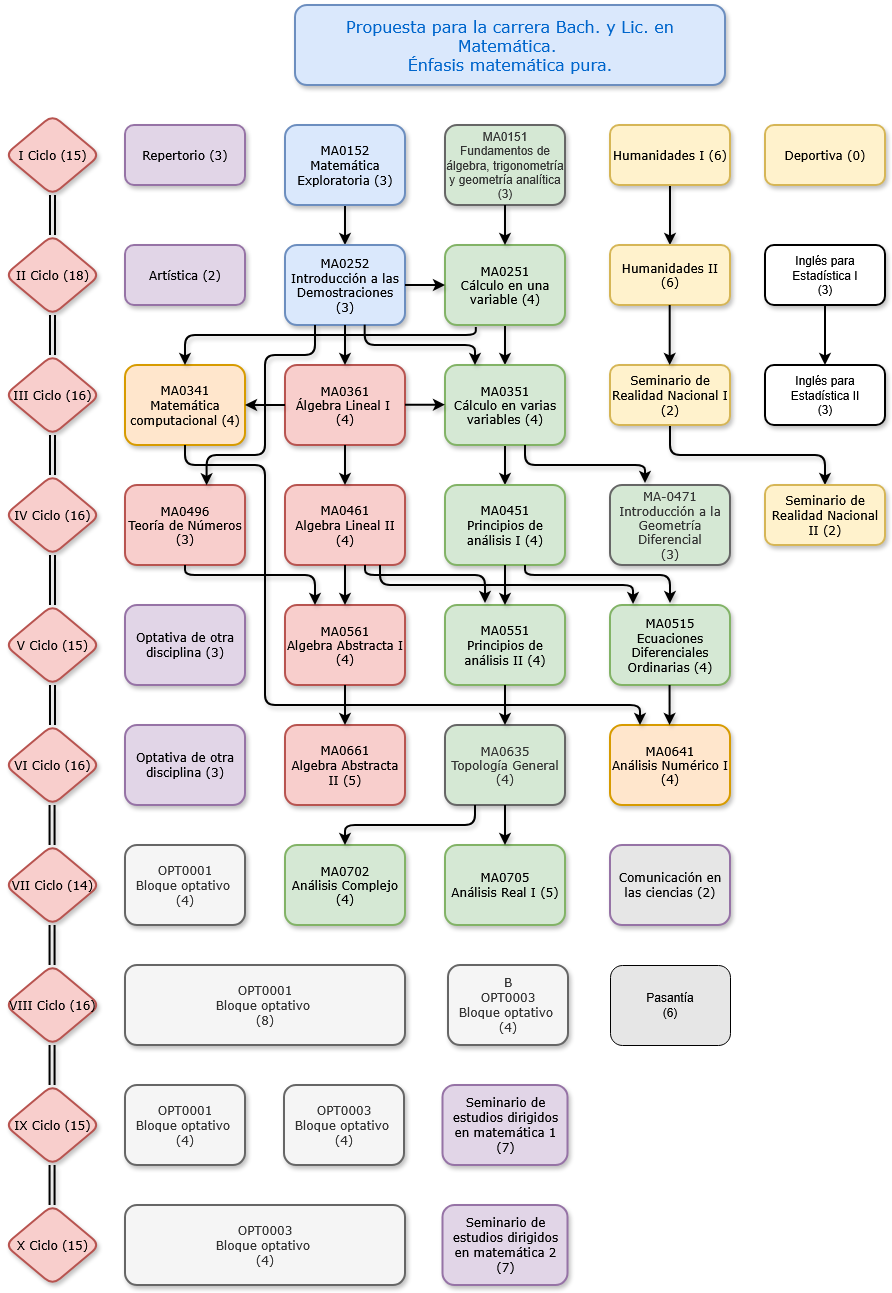
\includegraphics[width=0.75\textwidth]{propuesta_pura}
\caption{Diagrama de plan de Bachillerato y Licenciatura en Matemática con énfasis en Matemática Pura}
\end{figure}

\begin{figure}
\centering
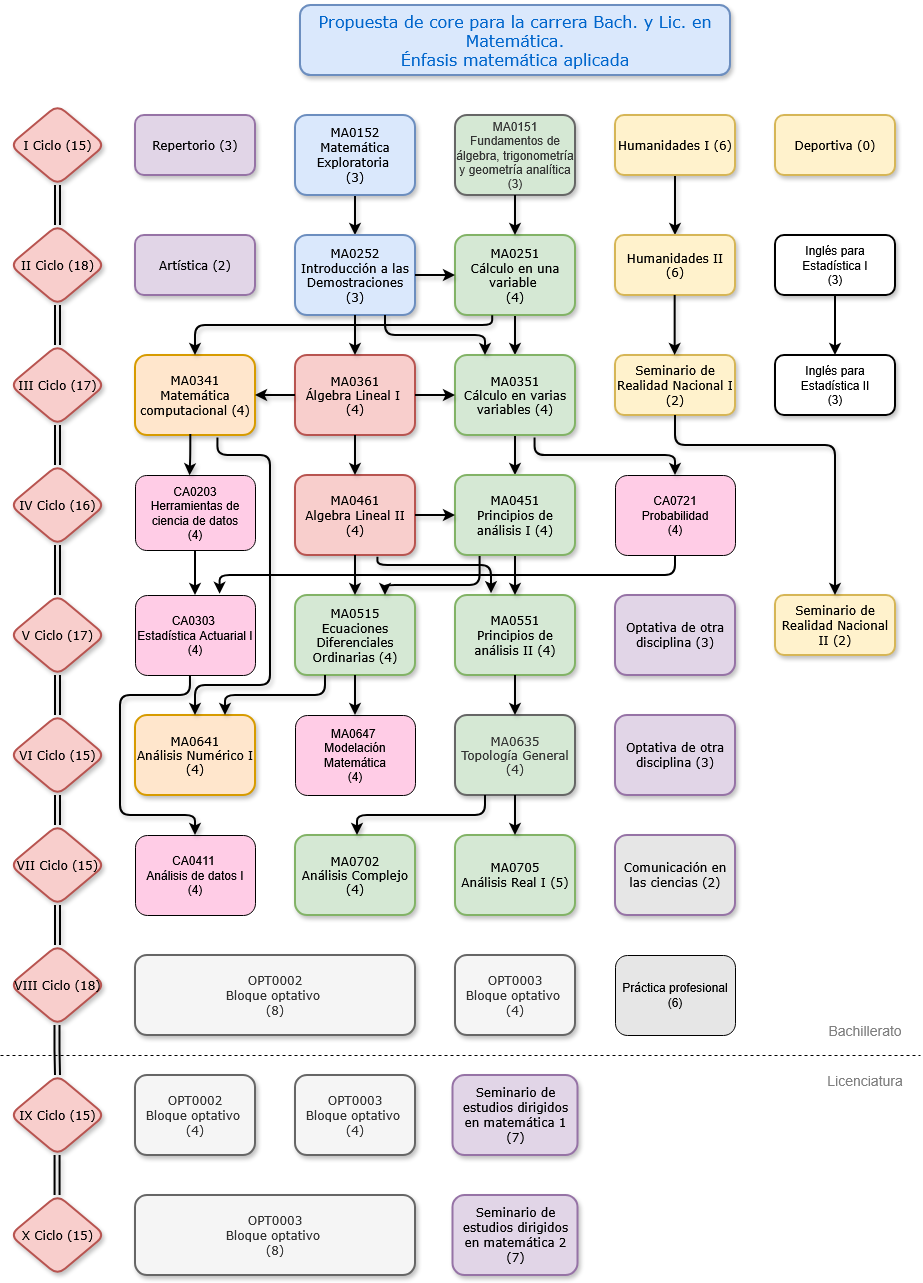
\includegraphics[width=0.75\textwidth]{propuesta_aplicada}
\caption{Diagrama de plan de Bachillerato y Licenciatura en Matemática con énfasis en Matemática Aplicada}
\end{figure}

\subsection{Requisitos de graduación}

\subsubsection{Bachillerato en matemática, ambos énfasis}

Se requiere de la asistencia, a lo largo de la carrera, a diez (10) actividades académicas válidas , por ejemplo:
\begin{enumerate}
    \item Charlas del Coloquio del Departamento de Matemáticas.
    \item Seminarios, conferencias o ciclos especiales anunciados por el departamento como válidos para este curso.
    \item Otras actividades académicas que la Dirección del Departamento disponga expresamente, con indicaciones oportunas.
\end{enumerate}

\subsubsection{Licenciatura en matemática, ambos énfasis}

Se requiere de la asistencia, a lo largo de la carrera, a cinco (5) actividades académicas válidas, distintas a las empleadas para cumplir el requerimiento similar de bachillerato, por ejemplo:
\begin{enumerate}
    \item Charlas del Coloquio del Departamento de Matemáticas.
    \item Seminarios, conferencias o ciclos especiales anunciados por el departamento como válidos para este curso.
    \item Otras actividades académicas que la Dirección del Departamento disponga expresamente, con indicaciones oportunas.
\end{enumerate}

\chapter{Programas de los cursos}

\section{Cursos}

En esta sección se incluye la lista de cursos de la propuesta, organizada por año y, cuando corresponde, por énfasis. Cada entrada enlaza al programa recogido en la sección~\ref{sec:anexo-programas}.

\subsection{Cursos de primer año}

La siguiente tabla muestra los niveles de dominio y contenidos esperados para estos dos semestres.

\begin{table}[H]
\begin{center}
\begin{tabular}{|ccc|}
\hline
\multicolumn{3}{|c|}{\cellcolor[HTML]{00C0F3} \textbf{Niveles de dominio y contenidos por área curricular}} \\ \hline
\multicolumn{1}{|l|}{\cellcolor[HTML]{8ED8F8}\textbf{Área curricular}} & \multicolumn{1}{l|}{\cellcolor[HTML]{8ED8F8}\textbf{Dominio}} & \cellcolor[HTML]{8ED8F8}\textbf{Contenidos} \\ \hline
\multicolumn{1}{|c|}{Habilidades operacionales} & \multicolumn{1}{c|}{Alto} & Alto \\ \hline
\multicolumn{1}{|l|}{Pensamiento abstracto} & \multicolumn{1}{c|}{Medio} & Bajo \\ \hline
\multicolumn{1}{|l|}{Pensamiento algorítmico} & \multicolumn{1}{c|}{Bajo} & Bajo \\ \hline
\multicolumn{1}{|l|}{Formalismo} & \multicolumn{1}{c|}{Bajo} & Bajo \\ \hline
\multicolumn{1}{|c|}{Habilidades investigativas} & \multicolumn{1}{c|}{-} & Bajo \\ \hline
\end{tabular}
\end{center}
\caption{Niveles de dominio y contenidos para los cursos del primer año de la carrera.}
\end{table}

\subsubsection*{Cursos comunes a los dos énfasis}

\begin{itemize}
    \item \hyperlink{MA0151}{MA-0151 Fundamentos de álgebra, trigonometría y geometría analítica}
    \item \hyperlink{MA0152}{MA-0152 Matemática Exploratoria}
    \item \hyperlink{MA0251}{MA-0251 Cálculo en una variable}
    \item \hyperlink{MA0252}{MA-0252 Introducción a las Demostraciones}
\end{itemize}


\subsection{Cursos de segundo año}

\begin{table}[H]
\begin{center}
\begin{tabular}{|ccc|}
\hline
\multicolumn{3}{|c|}{\cellcolor[HTML]{00C0F3} \textbf{Niveles de dominio y contenidos por área curricular}} \\ \hline
\multicolumn{1}{|l|}{\cellcolor[HTML]{8ED8F8}\textbf{Área curricular}} & \multicolumn{1}{l|}{\cellcolor[HTML]{8ED8F8}\textbf{Dominio}} & \cellcolor[HTML]{8ED8F8}\textbf{Contenidos} \\ \hline
\multicolumn{1}{|l|}{Habilidades operacionales} & \multicolumn{1}{c|}{Alto} & Medio \\ \hline
\multicolumn{1}{|l|}{Pensamiento abstracto} & \multicolumn{1}{c|}{Medio} & Medio \\ \hline
\multicolumn{1}{|l|}{Pensamiento algorítmico} & \multicolumn{1}{c|}{Medio} & Medio \\ \hline
\multicolumn{1}{|l|}{Formalismo} & \multicolumn{1}{c|}{Medio} & Medio \\ \hline
\multicolumn{1}{|l|}{Habilidades investigativas} & \multicolumn{1}{c|}{-} & Bajo \\ \hline
\end{tabular}
\end{center}
\caption{Niveles de dominio y contenidos para los cursos del segundo año de la carrera.}
\end{table}

\subsubsection*{Cursos comunes a los dos énfasis}

\begin{itemize}
    \item \hyperlink{MA0341}{MA-0341 Matemática Computacional}
    \item \hyperlink{MA0351}{MA-0351 Cálculo en varias variables}
    \item \hyperlink{MA0361}{MA-0361 Algebra Lineal I}
    \item \hyperlink{MA0451}{MA-0451 Principios de análisis I}
    \item \hyperlink{MA0461}{MA-0461 Algebra Lineal II}
\end{itemize}

\subsubsection*{Cursos del énfasis en matemática pura}
\begin{itemize}
    \item \hyperlink{MA0471}{MA-0471 Introducción a la Geometría Diferencial}
    \item \hyperlink{MA0496}{MA-0496 Teoría de Números}
\end{itemize}

\subsubsection*{Cursos del énfasis en matemática aplicada}
\begin{itemize}
    \item {CA-0204 Herramientas de ciencia de datos I}
    \item \hyperlink{CA0721}{CA-0721 Probabilidad}
\end{itemize}




\subsection{Cursos de tercer año}

La siguiente tabla resume los niveles de dominio y contenidos esperados para el tercer año, según las áreas curriculares definidas en este capítulo.

\begin{table}[H]
\begin{center}
\begin{tabular}{|ccc|}
\hline
\multicolumn{3}{|c|}{\cellcolor[HTML]{00C0F3} \textbf{Niveles de dominio y contenidos por área curricular}} \\ \hline
\multicolumn{1}{|l|}{\cellcolor[HTML]{8ED8F8}\textbf{Área curricular}} & \multicolumn{1}{l|}{\cellcolor[HTML]{8ED8F8}\textbf{Dominio}} & \cellcolor[HTML]{8ED8F8}\textbf{Contenidos} \\ \hline
\multicolumn{1}{|l|}{Habilidades operacionales} & \multicolumn{1}{c|}{Alto} & Bajo \\ \hline
\multicolumn{1}{|l|}{Pensamiento abstracto} & \multicolumn{1}{c|}{Alto} & Alto \\ \hline
\multicolumn{1}{|l|}{Pensamiento algorítmico} & \multicolumn{1}{c|}{Alto} & Alto \\ \hline
\multicolumn{1}{|l|}{Formalismo} & \multicolumn{1}{c|}{Alto} & Medio \\ \hline
\multicolumn{1}{|l|}{Habilidades investigativas} & \multicolumn{1}{c|}{Bajo} & Bajo \\ \hline
\end{tabular}
\end{center}
\caption{Niveles de dominio y contenidos para los cursos del tercer año de la carrera.}
\end{table}

\subsubsection*{Cursos comunes a los dos énfasis}

\begin{itemize}
    \item \hyperlink{MA0515}{MA-0515 Ecuaciones Diferenciales Ordinarias}
    \item \hyperlink{MA0551}{MA-0551 Principios de Análisis II}
    \item \hyperlink{MA0635}{MA-0635 Topología General}
    \item \hyperlink{MA0641}{MA-0641 Análisis Numérico I}
\end{itemize}

\subsubsection*{Cursos del énfasis en matemática pura}
\begin{itemize}
    \item \hyperlink{MA0561}{MA-0561 Algebra Abstracta I}
    \item \hyperlink{MA0661}{MA-0661 Algebra Abstracta II}
\end{itemize}

\subsubsection*{Cursos del énfasis en matemática aplicada}
\begin{itemize}
    \item {CA-0303 Estadística Actuarial I}
    \item \hyperlink{MA0647}{MA-0647 Modelación Matemática}
\end{itemize}

\subsection{Cursos de cuarto año}

La siguiente tabla resume los niveles de dominio y contenidos esperados para el cuarto año, según las áreas curriculares definidas en este capítulo.

\begin{table}[H]
\begin{center}
\begin{tabular}{|ccc|}
\hline
\multicolumn{3}{|c|}{\cellcolor[HTML]{00C0F3} \textbf{Niveles de dominio y contenidos por área curricular}} \\ \hline
\multicolumn{1}{|l|}{\cellcolor[HTML]{8ED8F8}\textbf{Área curricular}} & \multicolumn{1}{l|}{\cellcolor[HTML]{8ED8F8}\textbf{Dominio}} & \cellcolor[HTML]{8ED8F8}\textbf{Contenidos} \\ \hline
\multicolumn{1}{|l|}{Habilidades operacionales} & \multicolumn{1}{c|}{Alto} & Bajo \\ \hline
\multicolumn{1}{|l|}{Pensamiento abstracto} & \multicolumn{1}{c|}{Alto} & Alto \\ \hline
\multicolumn{1}{|l|}{Pensamiento algorítmico} & \multicolumn{1}{c|}{Alto} & Alto \\ \hline
\multicolumn{1}{|l|}{Formalismo} & \multicolumn{1}{c|}{Alto} & Alto \\ \hline
\multicolumn{1}{|l|}{Habilidades investigativas} & \multicolumn{1}{c|}{Medio} & Medio \\ \hline
\end{tabular}
\end{center}
\caption{Niveles de dominio y contenidos para los cursos del cuarto año de la carrera.}
\end{table}

\subsubsection*{Cursos comunes a los dos énfasis}

\begin{itemize}
    \item \hyperlink{MA0702}{MA-0702 Análisis Complejo}
    \item \hyperlink{MA0705}{MA-0705 Análisis Real I}
    \item \hyperlink{MA0880}{MA-0880 Comunicación en las ciencias}
\end{itemize}

\subsubsection*{Cursos del énfasis en matemática pura}
\begin{itemize}
    \item \hyperlink{MA0881Pura}{MA-0881 Práctica profesional en matemática pura}
\end{itemize}

\subsubsection*{Cursos del énfasis en matemática aplicada}
\begin{itemize}
    \item {CA-0411 Análisis de Datos I}
    \item \hyperlink{MA0883}{MA-0883 Práctica profesional en matemática aplicada}
\end{itemize}

\subsection{Cursos de licenciatura}

Las áreas curriculares del capítulo de estructura curricular contemplan explícitamente los años I a IV; para la licenciatura se proyecta la culminación de esa progresión, con énfasis reforzado en habilidades investigativas mediante los seminarios de estudios dirigidos.

\begin{table}[H]
\begin{center}
\begin{tabular}{|ccc|}
\hline
\multicolumn{3}{|c|}{\cellcolor[HTML]{00C0F3} \textbf{Niveles de dominio y contenidos por área curricular}} \\ \hline
\multicolumn{1}{|l|}{\cellcolor[HTML]{8ED8F8}\textbf{Área curricular}} & \multicolumn{1}{l|}{\cellcolor[HTML]{8ED8F8}\textbf{Dominio}} & \cellcolor[HTML]{8ED8F8}\textbf{Contenidos} \\ \hline
\multicolumn{1}{|l|}{Habilidades operacionales} & \multicolumn{1}{c|}{Alto} & Bajo \\ \hline
\multicolumn{1}{|l|}{Pensamiento abstracto} & \multicolumn{1}{c|}{Alto} & Alto \\ \hline
\multicolumn{1}{|l|}{Pensamiento algorítmico} & \multicolumn{1}{c|}{Alto} & Alto \\ \hline
\multicolumn{1}{|l|}{Formalismo} & \multicolumn{1}{c|}{Alto} & Alto \\ \hline
\multicolumn{1}{|l|}{Habilidades investigativas} & \multicolumn{1}{c|}{Alto} & Alto \\ \hline
\end{tabular}
\end{center}
\caption{Niveles de dominio y contenidos proyectados para los cursos de licenciatura.}
\end{table}

\subsubsection*{Énfasis en matemática pura}
\begin{itemize}
    \item \hyperlink{MA0982}{MA-0982 Seminario de estudios dirigidos en matemática pura I}
    \item \hyperlink{MA1081Pura}{MA-1081 Seminario de estudios dirigidos en matemática pura II}
\end{itemize}

\subsubsection*{Énfasis en matemática aplicada}
\begin{itemize}
    \item \hyperlink{MA0984}{MA-0984 Seminario de estudios dirigidos en matemática aplicada I}
    \item \hyperlink{MA1082}{MA-1082 Seminario de estudios dirigidos en matemática aplicada II}
\end{itemize}

\subsection{Cursos optativos}
\subsubsection*{Cursos optativos de núcleo en matemática pura OPT-001}

\begin{itemize}
    \item \hyperlink{MA0788}{MA-0788 Análisis Real II}
    \item \hyperlink{MA0506}{MA-0506 Teoría algebraica de números}
    \item \hyperlink{MA0809}{MA-0809 Teoría analítica de números}
    \item \hyperlink{MA0512}{MA-0512 Teoría de conjuntos}
    \item \hyperlink{MA0525}{MA-0525 Combinatoria}
    \item \hyperlink{MA0528}{MA-0528 Sistemas dinámicos}
    \item \hyperlink{MA0703}{MA-0703 Integración}
    \item \hyperlink{MA0707}{MA-0707 Geometría Diferencial}
    \item \hyperlink{MA0810}{MA-0810 Geometría algebraica I}
    \item \hyperlink{MA0711}{MA-0711 Lógica}
    \item \hyperlink{MA0714}{MA-0714 Optimización}
    \item \hyperlink{MA0755}{MA-0755 Ecuaciones diferenciales parciales}
    \item \hyperlink{MA0804}{MA-0804 Topología algebraica}
    \item \hyperlink{MA0806}{MA-0806 Análisis funcional}
    \item \hyperlink{MA0815}{MA-0815 Análisis armónico}
    \item \hyperlink{MA0820}{MA-0820 Teoría de modelos}
    \item \hyperlink{MA0840}{MA-0840 Probabilidad}
    \item \hyperlink{MA0860}{MA-0860 Teoría de módulos}
    \item \hyperlink{MA0889}{MA-0889 Álgebra conmutativa}
    \item \hyperlink{MA0920}{MA-0920 Ecuaciones en derivadas parciales numéricas}
\end{itemize}

\subsubsection*{Cursos optativos de núcleo en matemática pura OPT-002}
\begin{itemize}
    \item {CA-0304 Herramientas de ciencia de datos II}
    \item {CA-0411 Análisis de Datos II}
    \item {CA-0403 Estadística actuarial II}
    \item {CA-0512 Modelos Lineales}
    \item {CA-0612 Series de Tiempo}
    \item \hyperlink{MA0406}{MA-0406 Introducción a la optimización}
    \item {MA-0477 Ecuaciones Diferenciales Aplicadas}
    \item {MA-0722 Estadística Matemática I}
\end{itemize}

\subsubsection*{Cursos optativos en general OPT-003}


\begin{itemize}
    \item \hyperlink{MA0788}{MA-0788 Análisis Real II}
    \item \hyperlink{MA0506}{MA-0506 Teoría algebraica de números}
    \item \hyperlink{MA0809}{MA-0809 Teoría analítica de números}
    \item \hyperlink{MA0512}{MA-0512 Teoría de conjuntos}
    \item \hyperlink{MA0525}{MA-0525 Combinatoria}
    \item \hyperlink{MA0528}{MA-0528 Sistemas dinámicos}
    \item \hyperlink{MA0703}{MA-0703 Integración}
    \item \hyperlink{MA0707}{MA-0707 Geometría Diferencial}
    \item \hyperlink{MA0810}{MA-0810 Geometría algebraica I}
    \item \hyperlink{MA0711}{MA-0711 Lógica}
    \item \hyperlink{MA0714}{MA-0714 Optimización}
    \item \hyperlink{MA0755}{MA-0755 Ecuaciones diferenciales parciales}
    \item \hyperlink{MA0804}{MA-0804 Topología algebraica}
    \item \hyperlink{MA0806}{MA-0806 Análisis funcional}
    \item \hyperlink{MA0815}{MA-0815 Análisis armónico}
    \item \hyperlink{MA0820}{MA-0820 Teoría de modelos}
    \item \hyperlink{MA0840}{MA-0840 Probabilidad}
    \item \hyperlink{MA0860}{MA-0860 Teoría de módulos}
    \item \hyperlink{MA0889}{MA-0889 Álgebra conmutativa}
    \item \hyperlink{MA0920}{MA-0920 Ecuaciones en derivadas parciales numéricas}
    \item {CA-304 Herramientas de ciencia de datos II}
    \item {CA-0411 Análisis de Datos II}
    \item {CA-0403 Estadística actuarial II}
    \item {CA-0512 Modelos Lineales}
    \item {CA-0612 Series de Tiempo}
    \item \hyperlink{MA0406}{MA-0406 Introducción a la optimización}
    \item {MA-0477 Ecuaciones Diferenciales Aplicadas}
    \item {MA-0722 Estadística Matemática I}    
    \item \hyperlink{MA0809}{MA-0809 Teoría analítica de números}
    \item \hyperlink{MA0790}{MA-0790 Tópicos de análisis}
    \item \hyperlink{MA0791}{MA-0791 Tópicos de Probabilidad}
    \item \hyperlink{MA0792}{MA-0792 Tópicos de Ecuaciones diferenciales}
    \item \hyperlink{MA0793}{MA-0793 Tópicos de Geometría}
    \item \hyperlink{MA0794}{MA-0794 Tópicos de Modelación}
    \item \hyperlink{MA0796}{MA-0796 Tópicos de Álgebra}
    \item \hyperlink{MA0797}{MA-0797 Tópicos de Matemática discreta}
    \item \hyperlink{MA0830}{MA-0830 Tópicos de Teoría de Números}
    \item \hyperlink{MA0831}{MA-0831 Tópicos de Lógica}
    \item \hyperlink{MA0832}{MA-0832 Tópicos en Topología}
    \item \hyperlink{MA0918}{MA-0918 Procesos estocásticos}
    \item \hyperlink{MA0794}{MA-0794 Tópicos de Modelación}
    \item \hyperlink{MA0795}{MA-0795 Tópicos de Computación científica}
    \item \hyperlink{MA0798}{MA-0798 Tópicos de Análisis de datos}
    \item \hyperlink{MA0799}{MA-0799 Tópicos de Aprendizaje automático}
    \item {MA-0759 Tópicos de Matemática Financiera}
    \item \hyperlink{MA0917}{MA-0917 Estadística II}
    \item \hyperlink{MA0918}{MA-0918 Procesos estocásticos}
    \item {CA-917 Estadística matemática II}
    \item \hyperlink{MA0795}{MA-0795 Tópicos de Computación científica}
\end{itemize}




\chapter{Anexos}
\section{Anexo: Programas de cursos}
\label{sec:anexo-programas}

Los programas se presentan en orden alfabético según la sigla del curso.

\inputcurso{Cursos/CA0203-herramientas-ciencia-datos-i-cuerpo}
\inputcurso{Cursos/CA0303-estadistica-i-cuerpo}
\inputcurso{Cursos/CA0411-analisis-datos-i-cuerpo}
\inputcurso{Cursos/CA0721-probabilidad-cuerpo}
\inputcurso{Cursos/MA0151-fundamentos-cuerpo}
\inputcurso{Cursos/MA0152-matematica-exploratoria-cuerpo}
\inputcurso{Cursos/MA0251-calculo-una-variable-cuerpo}
\inputcurso{Cursos/MA0252-intro-demostraciones-cuerpo}
\inputcurso{Cursos/MA0341-matematica-computacional-i-cuerpo}
\inputcurso{Cursos/MA0351-calculo-varias-variables-cuerpo}
\inputcurso{Cursos/MA0361-algebra-lineal-i-cuerpo}
\inputcurso{Cursos/MA0406-introduccion-optimizacion-cuerpo}
\inputcurso{Cursos/MA0451-principios-analisis-i-cuerpo}
\inputcurso{Cursos/MA0461-algebra-lineal-ii-cuerpo}
\inputcurso{Cursos/MA0471-geometria-cuerpo}
\inputcurso{Cursos/MA0496-teoria-numeros-cuerpo}
\inputcurso{Cursos/MA0506-teoria-algebraica-numeros-cuerpo}
\inputcurso{Cursos/MA0512-teoria-conjuntos-cuerpo}
\inputcurso{Cursos/MA0515-ecuaciones-diferenciales-cuerpo}
\inputcurso{Cursos/MA0525-combinatoria-cuerpo}
\inputcurso{Cursos/MA0528-sistemas-dinamicos-cuerpo}
\inputcurso{Cursos/MA0551-principios-analisis-ii-cuerpo}
\inputcurso{Cursos/MA0561-algebra-abstracta-i-cuerpo}
\inputcurso{Cursos/MA0609-teoria-analitica-numeros-cuerpo}
\inputcurso{Cursos/MA0635-topologia-cuerpo}
\inputcurso{Cursos/MA0641-matematica-computacional-ii-cuerpo}
\inputcurso{Cursos/MA0647-modelacion-matematica-cuerpo}
\inputcurso{Cursos/MA0661-algebra-abstracta-ii-cuerpo}
\inputcurso{Cursos/MA0701-seminario-matematica-cuerpo}
\inputcurso{Cursos/MA0702-analisis-complejo-cuerpo}
\inputcurso{Cursos/MA0703-integracion-cuerpo}
\inputcurso{Cursos/MA0705-analisis-real-i-cuerpo}
\inputcurso{Cursos/MA0707-geometria-diferencial-cuerpo}
\inputcurso{Cursos/MA0709-geometria-algebraica-i-cuerpo}
\inputcurso{Cursos/MA0711-logica-cuerpo}
\inputcurso{Cursos/MA0714-optimizacion-cuerpo}
\inputcurso{Cursos/MA0755-ecuaciones-diferenciales-parciales-cuerpo}
\inputcurso{Cursos/MA0780-comunicacion-ciencias-cuerpo}
\inputcurso{Cursos/MA0781-practica-profesional-cuerpo}
\inputcurso{Cursos/MA0781-seminario-estudios-dirigidos-i-cuerpo}
\inputcurso{Cursos/MA0790-topicos-analisis-cuerpo}
\inputcurso{Cursos/MA0791-topicos-probabilidad-cuerpo}
\inputcurso{Cursos/MA0792-topicos-ecuaciones-diferenciales-cuerpo}
\inputcurso{Cursos/MA0793-topicos-geometria-cuerpo}
\inputcurso{Cursos/MA0794-topicos-modelacion-cuerpo}
\inputcurso{Cursos/MA0795-topicos-computacion-cientifica-cuerpo}
\inputcurso{Cursos/MA0796-topicos-algebra-cuerpo}
\inputcurso{Cursos/MA0797-topicos-matematica-discreta-cuerpo}
\inputcurso{Cursos/MA0798-topicos-analisis-datos-cuerpo}
\inputcurso{Cursos/MA0799-topicos-aprendizaje-automatico-cuerpo}
\inputcurso{Cursos/MA0804-topologia-algebraica-cuerpo}
\inputcurso{Cursos/MA0806-analisis-funcional-cuerpo}
\inputcurso{Cursos/MA0815-analisis-armonico-cuerpo}
\inputcurso{Cursos/MA0817-estadistica-matematica-i-cuerpo}
\inputcurso{Cursos/MA0820-teoria-modelos-cuerpo}
\inputcurso{Cursos/MA0830-topicos-teoria-numeros-cuerpo}
\inputcurso{Cursos/MA0831-topicos-logica-cuerpo}
\inputcurso{Cursos/MA0832-topicos-topologia-cuerpo}
\inputcurso{Cursos/MA0840-probabilidad-cuerpo}
\inputcurso{Cursos/MA0860-teoria-modulos-cuerpo}
\inputcurso{Cursos/MA0881-seminario-estudios-dirigidos-cuerpo}
\inputcurso{Cursos/MA0889-algebra-conmutativa-cuerpo}
\inputcurso{Cursos/MA0917-estadistica-matematica-ii-cuerpo}
\inputcurso{Cursos/MA0918-procesos-estocasticos-cuerpo}
\inputcurso{Cursos/MA0920-edp-numericas-cuerpo}
%\inputcurso{Cursos/CA0304-herramientas-ciencia-datos-ii-cuerpo}
%\inputcurso{Cursos/CA0412-analisis-datos-ii-cuerpo}
%\inputcurso{Cursos/CA0512-modelos-lineales-cuerpo}
%\inputcurso{Cursos/CA0612-series-tiempo-cuerpo}
%\newpage
Primer año

\begin{table}[H]
\begin{center}
\begin{tabular}{|ccc|}
\hline
\multicolumn{3}{|c|}{\cellcolor[HTML]{00C0F3} \textbf{Niveles de dominio y contenidos por área curricular}} \\ \hline
\multicolumn{1}{|l|}{Área curricular} & \multicolumn{1}{l|}{Alto} & Alto \\ \hline
\multicolumn{1}{|l|}{Habilidades operacionales} & \multicolumn{1}{l|}{Alto} & Alto \\ \hline
\multicolumn{1}{|l|}{Pensamiento abstracto} & \multicolumn{1}{l|}{Medio} & Bajo \\ \hline
\multicolumn{1}{|l|}{Pensamiento algorítmico} & \multicolumn{1}{l|}{Bajo} & Bajo \\ \hline
\multicolumn{1}{|l|}{Formalismo} & \multicolumn{1}{l|}{Bajo} & Bajo \\ \hline
\multicolumn{1}{|l|}{Habilidades investigativas} & \multicolumn{1}{l|}{-} & Bajo \\ \hline
\end{tabular}
\end{center}
\end{table}

Segundo año

\begin{table}[H]
\begin{center}
\begin{tabular}{|ccc|}
\hline
\multicolumn{3}{|c|}{\cellcolor[HTML]{00C0F3} \textbf{Niveles de dominio y contenidos por área curricular}} \\ \hline
\multicolumn{1}{|l|}{Área curricular} & \multicolumn{1}{l|}{Alto} & Alto \\ \hline
\multicolumn{1}{|l|}{Habilidades operacionales} & \multicolumn{1}{l|}{Alto} & Medio \\ \hline
\multicolumn{1}{|l|}{Pensamiento abstracto} & \multicolumn{1}{l|}{Medio} & Medio \\ \hline
\multicolumn{1}{|l|}{Pensamiento algorítmico} & \multicolumn{1}{l|}{Medio} & Medio \\ \hline
\multicolumn{1}{|l|}{Formalismo} & \multicolumn{1}{l|}{Medio} & Medio \\ \hline
\multicolumn{1}{|l|}{Habilidades investigativas} & \multicolumn{1}{l|}{-} & Bajo \\ \hline
\end{tabular}
\end{center}
\end{table}

tercer año

\begin{table}[H]
\begin{center}
\begin{tabular}{|ccc|}
\hline
\multicolumn{3}{|c|}{\cellcolor[HTML]{00C0F3}\textbf{Niveles de dominio y contenidos por área curricular}} \\ \hline
\multicolumn{1}{|l|}{Área curricular} & \multicolumn{1}{l|}{Alto} & Alto \\ \hline
\multicolumn{1}{|l|}{Habilidades operacionales} & \multicolumn{1}{l|}{Alto} & Bajo \\ \hline
\multicolumn{1}{|l|}{Pensamiento abstracto} & \multicolumn{1}{l|}{Alto} & Alto \\ \hline
\multicolumn{1}{|l|}{Pensamiento algorítmico} & \multicolumn{1}{l|}{Alto} & Alto \\ \hline
\multicolumn{1}{|l|}{Formalismo} & \multicolumn{1}{l|}{Alto} & Medio \\ \hline
\multicolumn{1}{|l|}{Habilidades investigativas} & \multicolumn{1}{l|}{Bajo} & Bajo \\ \hline
\end{tabular}
\end{center}
\end{table}

Cuarto año


\begin{table}[H]
\begin{center}
\begin{tabular}{|ccc|}
\hline
\multicolumn{3}{|c|}{\cellcolor[HTML]{00C0F3} \textbf{Niveles de dominio y contenidos por área curricular}} \\ \hline
\multicolumn{1}{|l|}{Área curricular} & \multicolumn{1}{l|}{Alto} & Alto \\ \hline
\multicolumn{1}{|l|}{Habilidades operacionales} & \multicolumn{1}{l|}{Alto} & Bajo \\ \hline
\multicolumn{1}{|l|}{Pensamiento abstracto} & \multicolumn{1}{l|}{Alto} & Alto \\ \hline
\multicolumn{1}{|l|}{Pensamiento algorítmico} & \multicolumn{1}{l|}{Alto} & Alto \\ \hline
\multicolumn{1}{|l|}{Formalismo} & \multicolumn{1}{l|}{Alto} & Alto \\ \hline
\multicolumn{1}{|l|}{Habilidades investigativas} & \multicolumn{1}{l|}{Medio} & Medio \\ \hline
\end{tabular}
\end{center}
\end{table}

\textbf{Reuniones sobre áreas disciplinares}

\begin{table}[H]
\begin{center}
\begin{tabular}{|llll|}
\hline
\multicolumn{4}{|c|}{\cellcolor[HTML]{00C0F3}\textbf{Cursos introductorios de demostraciones}} \\ \hline
\multicolumn{1}{|l|}{\begin{tabular}[c]{@{}l@{}}\cellcolor[HTML]{8ED8F8} \textbf{Fecha de}\\ \cellcolor[HTML]{8ED8F8} \textbf{reuniones}\end{tabular}} & \multicolumn{1}{l|}{\cellcolor[HTML]{8ED8F8} \textbf{Reuniones}} & \multicolumn{1}{l|}{\cellcolor[HTML]{8ED8F8}\textbf{Personas que asistieron}} & \begin{tabular}[c]{@{}l@{}}\cellcolor[HTML]{8ED8F8}\textbf{Resumen de} \\ \cellcolor[HTML]{8ED8F8} \textbf{temas discutidos}\end{tabular} \\ \hline
\multicolumn{1}{|l|}{} & \multicolumn{1}{l|}{} & \multicolumn{1}{l|}{\begin{tabular}[c]{@{}l@{}}\end{tabular}} &  \\ \hline
\multicolumn{1}{|l|}{} & \multicolumn{1}{l|}{} & \multicolumn{1}{l|}{} &  \\ \hline
\multicolumn{1}{|l|}{} & \multicolumn{1}{l|}{} & \multicolumn{1}{l|}{} &  \\ \hline
\multicolumn{1}{|l|}{} & \multicolumn{1}{l|}{} & \multicolumn{1}{l|}{} &  \\ \hline
\multicolumn{1}{|l|}{} & \multicolumn{1}{l|}{} & \multicolumn{1}{l|}{} &  \\ \hline
\end{tabular}
\end{center}
\end{table}

\begin{table}[H]
\begin{center}
\begin{tabular}{|llll|}
\hline
\multicolumn{4}{|c|}{\cellcolor[HTML]{00C0F3}\textbf{Álgebra}} \\ \hline
\multicolumn{1}{|l|}{\begin{tabular}[c]{@{}l@{}} \cellcolor[HTML]{8ED8F8}\textbf{Fecha de}\\ \cellcolor[HTML]{8ED8F8} \textbf{reuniones}\end{tabular}} & \multicolumn{1}{l|}{\cellcolor[HTML]{8ED8F8} \textbf{Reuniones}} & \multicolumn{1}{l|}{\cellcolor[HTML]{8ED8F8} \textbf{Personas que asistieron}} & \begin{tabular}[c]{@{}l@{}}\cellcolor[HTML]{8ED8F8} \textbf{Resumen de} \\ \cellcolor[HTML]{8ED8F8} \textbf{temas discutidos}\end{tabular} \\ \hline
\multicolumn{1}{|l|}{} & \multicolumn{1}{l|}{} & \multicolumn{1}{l|}{\begin{tabular}[c]{@{}l@{}}\end{tabular}} &  \\ \hline
\multicolumn{1}{|l|}{} & \multicolumn{1}{l|}{} & \multicolumn{1}{l|}{} &  \\ \hline
\multicolumn{1}{|l|}{} & \multicolumn{1}{l|}{} & \multicolumn{1}{l|}{} &  \\ \hline
\multicolumn{1}{|l|}{} & \multicolumn{1}{l|}{} & \multicolumn{1}{l|}{} &  \\ \hline
\multicolumn{1}{|l|}{} & \multicolumn{1}{l|}{} & \multicolumn{1}{l|}{} &  \\ \hline
\end{tabular}
\end{center}
\end{table}
\begin{table}[H]
\begin{center}
\begin{tabular}{|llll|}
\hline
\multicolumn{4}{|c|}{\cellcolor[HTML]{00C0F3}\textbf{Geometría y Topología}} \\ \hline
\multicolumn{1}{|l|}{\begin{tabular}[c]{@{}l@{}}\cellcolor[HTML]{8ED8F8} \textbf{Fecha de}\\ \cellcolor[HTML]{8ED8F8} \textbf{reuniones}\end{tabular}} & \multicolumn{1}{l|}{\cellcolor[HTML]{8ED8F8} \textbf{Reuniones}} & \multicolumn{1}{l|}{\cellcolor[HTML]{8ED8F8} \textbf{Personas que asistieron}} & \begin{tabular}[c]{@{}l@{}}\cellcolor[HTML]{8ED8F8} \textbf{Resumen de} \\ \cellcolor[HTML]{8ED8F8} \textbf{temas discutidos}\end{tabular} \\ \hline
\multicolumn{1}{|l|}{} & \multicolumn{1}{l|}{} & \multicolumn{1}{l|}{\begin{tabular}[c]{@{}l@{}}\end{tabular}} &  \\ \hline
\multicolumn{1}{|l|}{} & \multicolumn{1}{l|}{} & \multicolumn{1}{l|}{} &  \\ \hline
\multicolumn{1}{|l|}{} & \multicolumn{1}{l|}{} & \multicolumn{1}{l|}{} &  \\ \hline
\multicolumn{1}{|l|}{} & \multicolumn{1}{l|}{} & \multicolumn{1}{l|}{} &  \\ \hline
\multicolumn{1}{|l|}{} & \multicolumn{1}{l|}{} & \multicolumn{1}{l|}{} &  \\ \hline
\end{tabular}
\end{center}
\end{table}



\begin{table}[H]
\begin{center}
\begin{tabular}{|llll|}
\hline
\multicolumn{4}{|c|}{\cellcolor[HTML]{00C0F3}\textbf{Análisis}} \\ \hline
\multicolumn{1}{|l|}{\begin{tabular}[c]{@{}l@{}}\cellcolor[HTML]{8ED8F8}\textbf{Fecha de}\\ \cellcolor[HTML]{8ED8F8} \textbf{reuniones}\end{tabular}} & \multicolumn{1}{l|}{\cellcolor[HTML]{8ED8F8}\textbf{Reuniones}} & \multicolumn{1}{l|}{\cellcolor[HTML]{8ED8F8}\textbf{Personas que asistieron}} & \begin{tabular}[c]{@{}l@{}}\cellcolor[HTML]{8ED8F8} \textbf{Resumen de} \\ \cellcolor[HTML]{8ED8F8} \textbf{temas discutidos}\end{tabular} \\ \hline
\multicolumn{1}{|l|}{} & \multicolumn{1}{l|}{} & \multicolumn{1}{l|}{\begin{tabular}[c]{@{}l@{}}\end{tabular}} &  \\ \hline
\multicolumn{1}{|l|}{} & \multicolumn{1}{l|}{} & \multicolumn{1}{l|}{} &  \\ \hline
\multicolumn{1}{|l|}{} & \multicolumn{1}{l|}{} & \multicolumn{1}{l|}{} &  \\ \hline
\multicolumn{1}{|l|}{} & \multicolumn{1}{l|}{} & \multicolumn{1}{l|}{} &  \\ \hline
\multicolumn{1}{|l|}{} & \multicolumn{1}{l|}{} & \multicolumn{1}{l|}{} &  \\ \hline
\end{tabular}
\end{center}
\end{table}

\begin{table}[H]
\begin{center}
\begin{tabular}{|llll|}
\hline
\multicolumn{4}{|c|}{\cellcolor[HTML]{00C0F3}\textbf{Computación Científica, Matemática Aplicada y Análisis Numérico}} \\ \hline
\multicolumn{1}{|l|}{\begin{tabular}[c]{@{}l@{}}\cellcolor[HTML]{8ED8F8} \textbf{Fecha de}\\ \cellcolor[HTML]{8ED8F8} \textbf{reuniones}\end{tabular}} & \multicolumn{1}{l|}{\cellcolor[HTML]{8ED8F8} \textbf{Reuniones}} & \multicolumn{1}{l|}{\cellcolor[HTML]{8ED8F8} \textbf{Personas que asistieron}} & \begin{tabular}[c]{@{}l@{}} \cellcolor[HTML]{8ED8F8} \textbf{Resumen de} \\ \cellcolor[HTML]{8ED8F8} \textbf{temas discutidos}\end{tabular} \\ \hline
\multicolumn{1}{|l|}{} & \multicolumn{1}{l|}{} & \multicolumn{1}{l|}{\begin{tabular}[c]{@{}l@{}}\end{tabular}} &  \\ \hline
\multicolumn{1}{|l|}{} & \multicolumn{1}{l|}{} & \multicolumn{1}{l|}{} &  \\ \hline
\multicolumn{1}{|l|}{} & \multicolumn{1}{l|}{} & \multicolumn{1}{l|}{} &  \\ \hline
\multicolumn{1}{|l|}{} & \multicolumn{1}{l|}{} & \multicolumn{1}{l|}{} &  \\ \hline
\multicolumn{1}{|l|}{} & \multicolumn{1}{l|}{} & \multicolumn{1}{l|}{} &  \\ \hline
\end{tabular}
\end{center}
\end{table}
% Sin \begin{refsection}: la sección global (0) no tiene citas; un \printbibliography aquí duplicaba ruido o quedaba vacío.

\begin{table}[H]
\begin{tabular}{|lllll|}
\hline
\rowcolor[HTML]{00C0F3} 
\multicolumn{5}{|c|}{\cellcolor[HTML]{00C0F3}Reuniones de Áreas disciplinares} \\ \hline
\rowcolor[HTML]{8ED8F8} 
\multicolumn{1}{|l|}{\cellcolor[HTML]{8ED8F8}} & \multicolumn{1}{c|}{\cellcolor[HTML]{8ED8F8}\begin{tabular}[c]{@{}c@{}}Fecha de \\ reuniones\end{tabular}} & \multicolumn{1}{c|}{\cellcolor[HTML]{8ED8F8}Reuniones} & \multicolumn{1}{c|}{\cellcolor[HTML]{8ED8F8}\begin{tabular}[c]{@{}c@{}}Personas que \\ asistieron\end{tabular}} & \multicolumn{1}{c|}{\cellcolor[HTML]{8ED8F8}\begin{tabular}[c]{@{}c@{}}Resumen de \\ temas discutidos\end{tabular}} \\ \hline
\multicolumn{1}{|c|}{\cellcolor[HTML]{8ED8F8}} & \multicolumn{1}{l|}{} & \multicolumn{1}{l|}{} & \multicolumn{1}{l|}{} &  \\ \cline{2-5} 
\multicolumn{1}{|c|}{\cellcolor[HTML]{8ED8F8}} & \multicolumn{1}{l|}{} & \multicolumn{1}{l|}{} & \multicolumn{1}{l|}{} &  \\ \cline{2-5} 
\multicolumn{1}{|c|}{\cellcolor[HTML]{8ED8F8}} & \multicolumn{1}{l|}{} & \multicolumn{1}{l|}{} & \multicolumn{1}{l|}{} &  \\ \cline{2-5} 
\multicolumn{1}{|c|}{\cellcolor[HTML]{8ED8F8}} & \multicolumn{1}{l|}{} & \multicolumn{1}{l|}{} & \multicolumn{1}{l|}{} &  \\ \cline{2-5} 
\multicolumn{1}{|c|}{\multirow{-5}{*}{\cellcolor[HTML]{8ED8F8}\begin{tabular}[c]{@{}c@{}}Cursos\\ Introductorios\\ de \\ demostraciones\end{tabular}}} & \multicolumn{1}{l|}{} & \multicolumn{1}{l|}{} & \multicolumn{1}{l|}{} &  \\ \hline
\multicolumn{1}{|l|}{\cellcolor[HTML]{8ED8F8}} & \multicolumn{1}{l|}{} & \multicolumn{1}{l|}{} & \multicolumn{1}{l|}{} &  \\ \cline{2-5} 
\multicolumn{1}{|l|}{\cellcolor[HTML]{8ED8F8}} & \multicolumn{1}{l|}{} & \multicolumn{1}{l|}{} & \multicolumn{1}{l|}{} &  \\ \cline{2-5} 
\multicolumn{1}{|l|}{\cellcolor[HTML]{8ED8F8}} & \multicolumn{1}{l|}{} & \multicolumn{1}{l|}{} & \multicolumn{1}{l|}{} &  \\ \cline{2-5} 
\multicolumn{1}{|l|}{\cellcolor[HTML]{8ED8F8}} & \multicolumn{1}{l|}{} & \multicolumn{1}{l|}{} & \multicolumn{1}{l|}{} &  \\ \cline{2-5} 
\multicolumn{1}{|l|}{\multirow{-5}{*}{\cellcolor[HTML]{8ED8F8}Álgebra}} & \multicolumn{1}{l|}{} & \multicolumn{1}{l|}{} & \multicolumn{1}{l|}{} &  \\ \hline
\multicolumn{1}{|l|}{\cellcolor[HTML]{8ED8F8}} & \multicolumn{1}{l|}{} & \multicolumn{1}{l|}{} & \multicolumn{1}{l|}{} &  \\ \cline{2-5} 
\multicolumn{1}{|l|}{\cellcolor[HTML]{8ED8F8}} & \multicolumn{1}{l|}{} & \multicolumn{1}{l|}{} & \multicolumn{1}{l|}{} &  \\ \cline{2-5} 
\multicolumn{1}{|l|}{\cellcolor[HTML]{8ED8F8}} & \multicolumn{1}{l|}{} & \multicolumn{1}{l|}{} & \multicolumn{1}{l|}{} &  \\ \cline{2-5} 
\multicolumn{1}{|l|}{\cellcolor[HTML]{8ED8F8}} & \multicolumn{1}{l|}{} & \multicolumn{1}{l|}{} & \multicolumn{1}{l|}{} &  \\ \cline{2-5} 
\multicolumn{1}{|l|}{\multirow{-5}{*}{\cellcolor[HTML]{8ED8F8}\begin{tabular}[c]{@{}l@{}}Geometría y\\ Topología\end{tabular}}} & \multicolumn{1}{l|}{} & \multicolumn{1}{l|}{} & \multicolumn{1}{l|}{} &  \\ \hline
\multicolumn{1}{|l|}{\cellcolor[HTML]{8ED8F8}} & \multicolumn{1}{l|}{} & \multicolumn{1}{l|}{} & \multicolumn{1}{l|}{} &  \\ \cline{2-5} 
\multicolumn{1}{|l|}{\cellcolor[HTML]{8ED8F8}} & \multicolumn{1}{l|}{} & \multicolumn{1}{l|}{} & \multicolumn{1}{l|}{} &  \\ \cline{2-5} 
\multicolumn{1}{|l|}{\cellcolor[HTML]{8ED8F8}} & \multicolumn{1}{l|}{} & \multicolumn{1}{l|}{} & \multicolumn{1}{l|}{} &  \\ \cline{2-5} 
\multicolumn{1}{|l|}{\cellcolor[HTML]{8ED8F8}} & \multicolumn{1}{l|}{} & \multicolumn{1}{l|}{} & \multicolumn{1}{l|}{} &  \\ \cline{2-5} 
\multicolumn{1}{|l|}{\multirow{-5}{*}{\cellcolor[HTML]{8ED8F8}Análisis}} & \multicolumn{1}{l|}{} & \multicolumn{1}{l|}{} & \multicolumn{1}{l|}{} &  \\ \hline
\multicolumn{1}{|l|}{\cellcolor[HTML]{8ED8F8}} & \multicolumn{1}{l|}{} & \multicolumn{1}{l|}{} & \multicolumn{1}{l|}{} &  \\ \cline{2-5} 
\multicolumn{1}{|l|}{\cellcolor[HTML]{8ED8F8}} & \multicolumn{1}{l|}{} & \multicolumn{1}{l|}{} & \multicolumn{1}{l|}{} &  \\ \cline{2-5} 
\multicolumn{1}{|l|}{\cellcolor[HTML]{8ED8F8}} & \multicolumn{1}{l|}{} & \multicolumn{1}{l|}{} & \multicolumn{1}{l|}{} &  \\ \cline{2-5} 
\multicolumn{1}{|l|}{\cellcolor[HTML]{8ED8F8}} & \multicolumn{1}{l|}{} & \multicolumn{1}{l|}{} & \multicolumn{1}{l|}{} &  \\ \cline{2-5} 
\multicolumn{1}{|l|}{\cellcolor[HTML]{8ED8F8}} & \multicolumn{1}{l|}{} & \multicolumn{1}{l|}{} & \multicolumn{1}{l|}{} &  \\ \cline{2-5} 
\multicolumn{1}{|l|}{\multirow{-6}{*}{\cellcolor[HTML]{8ED8F8}\begin{tabular}[c]{@{}l@{}}Computación \\ Científica,\\ Matemática\\ Aplicada y\\ Análisis\\ Numérico\end{tabular}}} & \multicolumn{1}{l|}{} & \multicolumn{1}{l|}{} & \multicolumn{1}{l|}{} &  \\ \hline
\end{tabular}
\end{table}

\begin{table}[H]
\begin{tabular}{|llll|}
\hline
\rowcolor[HTML]{00C0F3} 
\multicolumn{4}{|l|}{\cellcolor[HTML]{00C0F3}\textbf{Cursos introductorios de demostraciones}} \\ \hline
\rowcolor[HTML]{8ED8F8}
\multicolumn{1}{|l|}{\cellcolor[HTML]{8ED8F8}\textbf{\begin{tabular}[c]{@{}l@{}}Fecha de \\ reunión\end{tabular}}} & \multicolumn{1}{l|}{\cellcolor[HTML]{8ED8F8}\textbf{Reuniones}} & \multicolumn{1}{c|}{\cellcolor[HTML]{8ED8F8}\textbf{\begin{tabular}[c]{@{}c@{}}Personas que\\ asistieron\end{tabular}}} & \multicolumn{1}{c|}{\cellcolor[HTML]{8ED8F8}\textbf{\begin{tabular}[c]{@{}c@{}}Resumen de \\ temas discutidos\end{tabular}}} \\ \hline
\multicolumn{1}{|l|}{} & \multicolumn{1}{l|}{} & \multicolumn{1}{l|}{} &  \\ \hline
\multicolumn{1}{|l|}{} & \multicolumn{1}{l|}{} & \multicolumn{1}{l|}{} &  \\ \hline
\multicolumn{1}{|l|}{} & \multicolumn{1}{l|}{} & \multicolumn{1}{l|}{} &  \\ \hline
\multicolumn{1}{|l|}{} & \multicolumn{1}{l|}{} & \multicolumn{1}{l|}{} &  \\ \hline
\multicolumn{1}{|l|}{} & \multicolumn{1}{l|}{} & \multicolumn{1}{l|}{} &  \\ \hline
\rowcolor[HTML]{00C0F3} 
\multicolumn{4}{|c|}{\cellcolor[HTML]{00C0F3}\textbf{Álgebra}} \\ \hline
\rowcolor[HTML]{8ED8F8}
\multicolumn{1}{|c|}{\cellcolor[HTML]{8ED8F8}\textbf{\begin{tabular}[c]{@{}c@{}}Fecha de \\ reuniones\end{tabular}}} & \multicolumn{1}{c|}{\cellcolor[HTML]{8ED8F8}\textbf{Reuniones}} & \multicolumn{1}{c|}{\cellcolor[HTML]{8ED8F8}\textbf{\begin{tabular}[c]{@{}c@{}}Personas que\\ asistieron\end{tabular}}} & \multicolumn{1}{c|}{\cellcolor[HTML]{8ED8F8}\textbf{\begin{tabular}[c]{@{}c@{}}Resumen de\\ temas discutidos\end{tabular}}} \\ \hline
\multicolumn{1}{|l|}{} & \multicolumn{1}{l|}{} & \multicolumn{1}{l|}{} &  \\ \hline
\multicolumn{1}{|l|}{} & \multicolumn{1}{l|}{} & \multicolumn{1}{l|}{} &  \\ \hline
\multicolumn{1}{|l|}{} & \multicolumn{1}{l|}{} & \multicolumn{1}{l|}{} &  \\ \hline
\multicolumn{1}{|l|}{} & \multicolumn{1}{l|}{} & \multicolumn{1}{l|}{} &  \\ \hline
\multicolumn{1}{|l|}{} & \multicolumn{1}{l|}{} & \multicolumn{1}{l|}{} &  \\ \hline
\rowcolor[HTML]{00C0F3} 
\multicolumn{4}{|c|}{\cellcolor[HTML]{00C0F3}\textbf{Geometría y Topología}} \\ \hline
\rowcolor[HTML]{8ED8F8}
\multicolumn{1}{|c|}{\cellcolor[HTML]{8ED8F8}\textbf{\begin{tabular}[c]{@{}c@{}}Fecha de \\ reuniones\end{tabular}}} & \multicolumn{1}{c|}{\cellcolor[HTML]{8ED8F8}\textbf{Reuniones}} & \multicolumn{1}{c|}{\cellcolor[HTML]{8ED8F8}\textbf{\begin{tabular}[c]{@{}c@{}}Personas que \\ asistieron\end{tabular}}} & \multicolumn{1}{c|}{\cellcolor[HTML]{8ED8F8}\textbf{\begin{tabular}[c]{@{}c@{}}Resumen de\\  temas discutidos\end{tabular}}} \\ \hline
\multicolumn{1}{|l|}{} & \multicolumn{1}{l|}{} & \multicolumn{1}{l|}{} &  \\ \hline
\multicolumn{1}{|l|}{} & \multicolumn{1}{l|}{} & \multicolumn{1}{l|}{} &  \\ \hline
\multicolumn{1}{|l|}{} & \multicolumn{1}{l|}{} & \multicolumn{1}{l|}{} &  \\ \hline
\multicolumn{1}{|l|}{} & \multicolumn{1}{l|}{} & \multicolumn{1}{l|}{} &  \\ \hline
\multicolumn{1}{|l|}{} & \multicolumn{1}{l|}{} & \multicolumn{1}{l|}{} &  \\ \hline
\rowcolor[HTML]{00C0F3} 
\multicolumn{4}{|c|}{\cellcolor[HTML]{00C0F3}\textbf{Ánalisis}} \\ \hline
\rowcolor[HTML]{8ED8F8}
\multicolumn{1}{|c|}{\cellcolor[HTML]{8ED8F8}\textbf{\begin{tabular}[c]{@{}c@{}}Fecha de \\ reuniones\end{tabular}}} & \multicolumn{1}{c|}{\cellcolor[HTML]{8ED8F8}\textbf{Reuniones}} & \multicolumn{1}{c|}{\cellcolor[HTML]{8ED8F8}\textbf{\begin{tabular}[c]{@{}c@{}}Personas que\\ asistieron\end{tabular}}} & \multicolumn{1}{c|}{\cellcolor[HTML]{8ED8F8}\textbf{\begin{tabular}[c]{@{}c@{}}Resumen de\\ temas discutidos\end{tabular}}} \\ \hline
\multicolumn{1}{|l|}{} & \multicolumn{1}{l|}{} & \multicolumn{1}{l|}{} &  \\ \hline
\multicolumn{1}{|l|}{} & \multicolumn{1}{l|}{} & \multicolumn{1}{l|}{} &  \\ \hline
\multicolumn{1}{|l|}{} & \multicolumn{1}{l|}{} & \multicolumn{1}{l|}{} &  \\ \hline
\multicolumn{1}{|l|}{} & \multicolumn{1}{l|}{} & \multicolumn{1}{l|}{} &  \\ \hline
\multicolumn{1}{|l|}{} & \multicolumn{1}{l|}{} & \multicolumn{1}{l|}{} &  \\ \hline
\rowcolor[HTML]{00C0F3} 
\multicolumn{4}{|c|}{\cellcolor[HTML]{00C0F3}\textbf{Computación Científica, Matemática Aplicada y Análisis Numérico}} \\ \hline
\rowcolor[HTML]{8ED8F8}
\multicolumn{1}{|c|}{\cellcolor[HTML]{8ED8F8}\textbf{\begin{tabular}[c]{@{}c@{}}Fecha de \\ reuniones\end{tabular}}} & \multicolumn{1}{c|}{\cellcolor[HTML]{8ED8F8}\textbf{Reuniones}} & \multicolumn{1}{c|}{\cellcolor[HTML]{8ED8F8}\textbf{\begin{tabular}[c]{@{}c@{}}Personas que \\ asistieron\end{tabular}}} & \multicolumn{1}{c|}{\cellcolor[HTML]{8ED8F8}\textbf{\begin{tabular}[c]{@{}c@{}}Resumen de \\ temas discutidos\end{tabular}}} \\ \hline
\multicolumn{1}{|l|}{} & \multicolumn{1}{l|}{} & \multicolumn{1}{l|}{} &  \\ \hline
\multicolumn{1}{|l|}{} & \multicolumn{1}{l|}{} & \multicolumn{1}{l|}{} &  \\ \hline
\multicolumn{1}{|l|}{} & \multicolumn{1}{l|}{} & \multicolumn{1}{l|}{} &  \\ \hline
\multicolumn{1}{|l|}{} & \multicolumn{1}{l|}{} & \multicolumn{1}{l|}{} &  \\ \hline
\multicolumn{1}{|l|}{} & \multicolumn{1}{l|}{} & \multicolumn{1}{l|}{} &  \\ \hline
\end{tabular}
\end{table}

\textbf{Reuniones de comité}

\begin{table}[H]
\begin{center}
\begin{tabular}{|lll|}
\hline
\rowcolor[HTML]{00C0F3} 
\multicolumn{3}{|c|}{\cellcolor[HTML]{00C0F3}Reuniones de comité} \\ \hline
\rowcolor[HTML]{8ED8F8}
\multicolumn{1}{|c|}{\cellcolor[HTML]{8ED8F8}Miembros de comité} & \multicolumn{1}{c|}{\cellcolor[HTML]{8ED8F8}\begin{tabular}[c]{@{}c@{}}Número de \\ reunión\end{tabular}} & \multicolumn{1}{c|}{\cellcolor[HTML]{8ED8F8}\begin{tabular}[c]{@{}c@{}}Horas reunidas\end{tabular}} \\ \hline
\multicolumn{1}{|l|}{} & \multicolumn{1}{l|}{} &  \\ \hline
\multicolumn{1}{|l|}{} & \multicolumn{1}{l|}{} &  \\ \hline
\multicolumn{1}{|l|}{} & \multicolumn{1}{l|}{} &  \\ \hline
\multicolumn{1}{|l|}{} & \multicolumn{1}{l|}{} &  \\ \hline
\multicolumn{1}{|l|}{} & \multicolumn{1}{l|}{} &  \\ \hline
\multicolumn{1}{|l|}{} & \multicolumn{1}{l|}{} &  \\ \hline
\multicolumn{1}{|l|}{} & \multicolumn{1}{l|}{} &  \\ \hline
\multicolumn{1}{|l|}{} & \multicolumn{1}{l|}{} &  \\ \hline
\end{tabular}
\end{center}
\end{table}


\begin{table}[]
\begin{tabular}{|ll|}
\hline
\rowcolor[HTML]{00C0F3} 
\multicolumn{2}{|c|}{\cellcolor[HTML]{00C0F3}} \\
\rowcolor[HTML]{00C0F3} 
\multicolumn{2}{|c|}{\cellcolor[HTML]{00C0F3}} \\
\rowcolor[HTML]{00C0F3} 
\multicolumn{2}{|c|}{\multirow{-3}{*}{\cellcolor[HTML]{00C0F3}\textbf{\begin{tabular}[c]{@{}c@{}}Objetivo 2.1: Conocer los principales tipos de Geometría para visualizar\\ los espacios euclídeos, hiperbólicos, esféricos y proyectivos.\end{tabular}}}} \\ \hline
\rowcolor[HTML]{8ED8F8} 
\multicolumn{1}{|c|}{\cellcolor[HTML]{8ED8F8}\textbf{Acciones}} & \multicolumn{1}{c|}{\cellcolor[HTML]{8ED8F8}\textbf{\begin{tabular}[c]{@{}c@{}}Estrategias metodológicas \\ \\ y tecnológicas\end{tabular}}} \\ \hline
\multicolumn{1}{|l|}{\begin{tabular}[c]{@{}l@{}}Estudiar las bases de la geometría clásica\\ (euclidiana).\end{tabular}} &  \\
\multicolumn{1}{|l|}{\begin{tabular}[c]{@{}l@{}}Estudiar las bases de Álgebra y Análisis real\\ y complejo\end{tabular}} & Exploración bibliográfica y web \\
\multicolumn{1}{|l|}{Estudiar la geometría proyectiva real y compleja.} & Resolución de ejercicios \\
\multicolumn{1}{|l|}{Reconocer los diferentes tipos de geometría.} & Trabajo en equipo \\
\multicolumn{1}{|l|}{Enfocar una o algunas ramas de preferencia.} &  \\ \hline
\rowcolor[HTML]{00C0F3} 
\multicolumn{2}{|c|}{\cellcolor[HTML]{00C0F3}} \\
\rowcolor[HTML]{00C0F3} 
\multicolumn{2}{|c|}{\cellcolor[HTML]{00C0F3}} \\
\rowcolor[HTML]{00C0F3} 
\multicolumn{2}{|c|}{\multirow{-3}{*}{\cellcolor[HTML]{00C0F3}\textbf{\begin{tabular}[c]{@{}c@{}}Objetivo 2.2: Conocer las propiedades de curvas, superficies y variedades para visualizar \\ las nociones geométricas básicas en espacios de dos, tres y más dimensiones.\\ .\end{tabular}}}} \\ \hline
\rowcolor[HTML]{8ED8F8} 
\multicolumn{1}{|c|}{\cellcolor[HTML]{8ED8F8}\textbf{Acciones}} & \multicolumn{1}{c|}{\cellcolor[HTML]{8ED8F8}\textbf{\begin{tabular}[c]{@{}c@{}}Estrategias metodológicas \\ \\ y tecnológicas\end{tabular}}} \\ \hline
\multicolumn{1}{|l|}{Estudiar las propiedades conocidas} &  \\
\multicolumn{1}{|l|}{\begin{tabular}[c]{@{}l@{}}Estudiar objetos asociados a las estructuras \\ geométricas (haces, fibrados vectoriales, \\ curvaturas).\end{tabular}} & Resolución de ejercicios \\
\multicolumn{1}{|l|}{\begin{tabular}[c]{@{}l@{}}Indagar los métodos y técnicas de estudio para \\ resolver los problemas geométricos.\end{tabular}} & \begin{tabular}[c]{@{}l@{}}Interacción con expertos de otras\\ áreas\end{tabular} \\ \hline
\rowcolor[HTML]{00C0F3} 
\multicolumn{2}{|c|}{\cellcolor[HTML]{00C0F3}} \\
\rowcolor[HTML]{00C0F3} 
\multicolumn{2}{|c|}{\cellcolor[HTML]{00C0F3}} \\
\rowcolor[HTML]{00C0F3} 
\multicolumn{2}{|c|}{\multirow{-3}{*}{\cellcolor[HTML]{00C0F3}\textbf{\begin{tabular}[c]{@{}c@{}}Objetivo 2.3: Resolver problemas de las estructuras geométricas\\ \\ para producir nuevo conocimiento.\end{tabular}}}} \\ \hline
\rowcolor[HTML]{8ED8F8} 
\multicolumn{1}{|c|}{\cellcolor[HTML]{8ED8F8}\textbf{\begin{tabular}[c]{@{}c@{}}.\\ Acciones\\ .\end{tabular}}} & \multicolumn{1}{c|}{\cellcolor[HTML]{8ED8F8}\textbf{\begin{tabular}[c]{@{}c@{}}.\\ Estrategias metodológicas \\ y tecnológicas\\ .\end{tabular}}} \\ \hline
\multicolumn{1}{|l|}{Reconocer el problema por resolver} & Exploración bibliográfica \\
\multicolumn{1}{|l|}{\begin{tabular}[c]{@{}l@{}}Identificar aplicaciones a otros problemas en \\ Geometría, otras áreas de la Matemática o en \\ la vida real.\end{tabular}} & \begin{tabular}[c]{@{}l@{}}Interacción con expertos de otras\\ \\  áreas.\end{tabular} \\
\multicolumn{1}{|l|}{\begin{tabular}[c]{@{}l@{}}Entender los pasos sucesivos al problema que\\ se trata de resolver.\end{tabular}} & Seminario, charlas. \\
\multicolumn{1}{|l|}{\begin{tabular}[c]{@{}l@{}}Plantear las técnicas necesarias para resolver el\\  problema\end{tabular}} &  \\ \hline
\rowcolor[HTML]{00C0F3} 
\multicolumn{2}{|c|}{\cellcolor[HTML]{00C0F3}} \\
\rowcolor[HTML]{00C0F3} 
\multicolumn{2}{|c|}{\cellcolor[HTML]{00C0F3}} \\
\rowcolor[HTML]{00C0F3} 
\multicolumn{2}{|c|}{\multirow{-3}{*}{\cellcolor[HTML]{00C0F3}\textbf{\begin{tabular}[c]{@{}c@{}}Objetivo 2.4: Investigar problemas en geometría para desarrollar\\ aplicaciones a problemas reales.\end{tabular}}}} \\ \hline
\rowcolor[HTML]{8ED8F8} 
\multicolumn{1}{|c|}{\cellcolor[HTML]{8ED8F8}\textbf{Acciones}} & \multicolumn{1}{c|}{\cellcolor[HTML]{8ED8F8}\textbf{\begin{tabular}[c]{@{}c@{}}Estrategias metodológicas\\ \\  y tecnológicas\end{tabular}}} \\ \hline
\multicolumn{1}{|l|}{\begin{tabular}[c]{@{}l@{}}Estudiar modelos geométricos de problemas \\ reales abiertos.\end{tabular}} &  \\
\multicolumn{1}{|l|}{\begin{tabular}[c]{@{}l@{}}Interactuar con profesionales de otras \\ disciplinas.\end{tabular}} & Visualización. \\
\multicolumn{1}{|l|}{Encriptar la información.} & Sofware especializado. \\
\multicolumn{1}{|l|}{Simplificar el problema para que sea aplicable.} & Interacción con otras disciplinas. \\
\multicolumn{1}{|l|}{\begin{tabular}[c]{@{}l@{}}Describir el problema mediante números que \\ puedan ser insertados en un sistema.\end{tabular}} &  \\ \hline
\rowcolor[HTML]{00C0F3} 
\multicolumn{2}{|c|}{\cellcolor[HTML]{00C0F3}} \\
\rowcolor[HTML]{00C0F3} 
\multicolumn{2}{|c|}{\cellcolor[HTML]{00C0F3}} \\
\rowcolor[HTML]{00C0F3} 
\multicolumn{2}{|c|}{\multirow{-3}{*}{\cellcolor[HTML]{00C0F3}\textbf{\begin{tabular}[c]{@{}c@{}}Objetivo 2.5: Divulgar la producción de conocimientos, para que \\ pueda ser comprendida y usada\end{tabular}}}} \\ \hline
\rowcolor[HTML]{8ED8F8} 
\multicolumn{1}{|c|}{\cellcolor[HTML]{8ED8F8}\textbf{Acciones}} & \multicolumn{1}{c|}{\cellcolor[HTML]{8ED8F8}\textbf{\begin{tabular}[c]{@{}c@{}}Estrategias metodológicas \\ y tecnológicas.\end{tabular}}} \\ \hline
\multicolumn{1}{|l|}{Elaborar documentos formales} & \begin{tabular}[c]{@{}l@{}}Uso de software especializado para\\ redactar artículos cienctíficos.\end{tabular} \\
\multicolumn{1}{|l|}{\begin{tabular}[c]{@{}l@{}}Socializar los conocimientos mediante la \\ interacción con otros profesionales.\end{tabular}} & \begin{tabular}[c]{@{}l@{}}Asistencia a conferencias, congresos,\\ seminarios, etc.\end{tabular} \\
\multicolumn{1}{|l|}{\begin{tabular}[c]{@{}l@{}}Comunicar los resultados mediante un \\ lenguaje interdisciplinario.\end{tabular}} & Realizar informes y presentaciones. \\ \hline
\end{tabular}
\end{table}



\begin{table}[]
\begin{tabular}{|ll|}
\hline
\rowcolor[HTML]{00C0F3} 
\multicolumn{2}{|c|}{\cellcolor[HTML]{00C0F3}} \\
\rowcolor[HTML]{00C0F3} 
\multicolumn{2}{|c|}{\cellcolor[HTML]{00C0F3}} \\
\rowcolor[HTML]{00C0F3} 
\multicolumn{2}{|c|}{\multirow{-3}{*}{\cellcolor[HTML]{00C0F3}\textbf{\begin{tabular}[c]{@{}c@{}}Objetivo 3.1: Demostrar nuevos resultados para contribuir en el entorno\\ \\ cient'ifico y social.\end{tabular}}}} \\ \hline
\rowcolor[HTML]{8ED8F8} 
\multicolumn{1}{|c|}{\cellcolor[HTML]{8ED8F8}\textbf{Acciones}} & \multicolumn{1}{c|}{\cellcolor[HTML]{8ED8F8}\textbf{\begin{tabular}[c]{@{}c@{}}Estrategias metodológicas \\ \\ y tecnológicas\end{tabular}}} \\ \hline
\multicolumn{1}{|l|}{Conocer las definiciones y los principios básicos.} &  \\ \hline
\multicolumn{1}{|l|}{Generalizar resultados, nociones y definiciones.} & Exploración bibliográfica y web \\ \hline
\multicolumn{1}{|l|}{Relacionar distintas áreas de la Teoría de Números} & Resolución de ejercicios. \\ \hline
\multicolumn{1}{|l|}{Efectuar cálculos concretos.} & Trabajo en equipo. \\ \hline
\rowcolor[HTML]{00C0F3} 
\multicolumn{2}{|c|}{\cellcolor[HTML]{00C0F3}} \\
\rowcolor[HTML]{00C0F3} 
\multicolumn{2}{|c|}{\cellcolor[HTML]{00C0F3}} \\
\rowcolor[HTML]{00C0F3} 
\multicolumn{2}{|c|}{\multirow{-3}{*}{\cellcolor[HTML]{00C0F3}\textbf{\begin{tabular}[c]{@{}c@{}}Objetivo 3.2: Conocer las propiedades de curvas, superficies y variedades para visualizar \\ las nociones geométricas básicas en espacios de dos, tres y más dimensiones.\\ .\end{tabular}}}} \\ \hline
\rowcolor[HTML]{8ED8F8} 
\multicolumn{1}{|c|}{\cellcolor[HTML]{8ED8F8}\textbf{Acciones}} & \multicolumn{1}{c|}{\cellcolor[HTML]{8ED8F8}\textbf{\begin{tabular}[c]{@{}c@{}}Estrategias metodológicas \\ \\ y tecnológicas\end{tabular}}} \\ \hline
\multicolumn{1}{|l|}{Elaborar algoritmos.} &  \\ \hline
\multicolumn{1}{|l|}{Analizar datos obtenidos.} & CAS \\ \hline
\multicolumn{1}{|l|}{\begin{tabular}[c]{@{}l@{}}Identificar patrones, tendencias y \\ comportamientos.\end{tabular}} & Lenguajes de programación. \\ \hline
\multicolumn{1}{|l|}{Implementar los algoritmos.} & \begin{tabular}[c]{@{}l@{}}Sistemas de cómputo especializados\\ en Teoría de Números.\end{tabular} \\ \hline
\rowcolor[HTML]{00C0F3} 
\multicolumn{2}{|c|}{\cellcolor[HTML]{00C0F3}} \\
\rowcolor[HTML]{00C0F3} 
\multicolumn{2}{|c|}{\cellcolor[HTML]{00C0F3}} \\
\rowcolor[HTML]{00C0F3} 
\multicolumn{2}{|c|}{\multirow{-3}{*}{\cellcolor[HTML]{00C0F3}\textbf{\begin{tabular}[c]{@{}c@{}}Objetivo 3.3: Formular conjeturas con base en observaciones experimentales\\ o teóricas sobre resultados plausibles para producir nuevo conocimiento.\end{tabular}}}} \\ \hline
\rowcolor[HTML]{8ED8F8} 
\multicolumn{1}{|c|}{\cellcolor[HTML]{8ED8F8}\textbf{Acciones}} & \multicolumn{1}{c|}{\cellcolor[HTML]{8ED8F8}\textbf{\begin{tabular}[c]{@{}c@{}}Estrategias metodológicas \\ y tecnológicas\end{tabular}}} \\ \hline
\multicolumn{1}{|l|}{Plantear problemas de estudio.} &  \\ \hline
\multicolumn{1}{|l|}{Generalizar resultados previamente encontrados.} & Exploración bibliográfica. \\ \hline
\multicolumn{1}{|l|}{Inducir resultados con base en la experimentación.} & \begin{tabular}[c]{@{}l@{}}Interacción con expertos de otras\\ áreas.\end{tabular} \\ \hline
\multicolumn{1}{|l|}{\begin{tabular}[c]{@{}l@{}}Ordenar resultados relacionados por medio de \\ puntos de vista unificadores.\end{tabular}} & Seminarios, charlas. \\ \hline
\rowcolor[HTML]{00C0F3} 
\multicolumn{2}{|c|}{\cellcolor[HTML]{00C0F3}} \\
\rowcolor[HTML]{00C0F3} 
\multicolumn{2}{|c|}{\cellcolor[HTML]{00C0F3}} \\
\rowcolor[HTML]{00C0F3} 
\multicolumn{2}{|c|}{\multirow{-3}{*}{\cellcolor[HTML]{00C0F3}\textbf{\begin{tabular}[c]{@{}c@{}}Objetivo 3.4: Demostrar nuevos resultados para contribuir en el\\ entorno científico y social.\end{tabular}}}} \\ \hline
\rowcolor[HTML]{8ED8F8} 
\multicolumn{1}{|c|}{\cellcolor[HTML]{8ED8F8}\textbf{Acciones}} & \multicolumn{1}{c|}{\cellcolor[HTML]{8ED8F8}\textbf{\begin{tabular}[c]{@{}c@{}}Estrategias metodológicas\\ \\  y tecnológicas\end{tabular}}} \\ \hline
\multicolumn{1}{|l|}{\begin{tabular}[c]{@{}l@{}}Estudiar modelos geométricos de problemas \\ reales abiertos.\end{tabular}} & \begin{tabular}[c]{@{}l@{}}Uso de software especializado como\\ CAS para ayudar en demostraciones \\ que involucran cálculos complicados.\end{tabular} \\ \hline
\multicolumn{1}{|l|}{\begin{tabular}[c]{@{}l@{}}Estudiar y aplicar las técnicas previas relacionadas\\ a los objetos estudiados.\end{tabular}} & \begin{tabular}[c]{@{}l@{}}Aplicación de técnicas usuales en el\\ estudio de los objetos particulares.\end{tabular} \\ \hline
\multicolumn{1}{|l|}{Crear nuevas teorías, conceptos y técnicas.} & \begin{tabular}[c]{@{}l@{}}Búsqueda de nuevos métodos para\\ solventar problemas nuevos.\end{tabular} \\ \hline
\multicolumn{1}{|l|}{Verificar y validar los teoremas obtenidos.} & \begin{tabular}[c]{@{}l@{}}Utilización de avances recientes para\\ demostrar nuevos teoremas.\end{tabular} \\ \hline
\multicolumn{1}{|l|}{} & \begin{tabular}[c]{@{}l@{}}Uso de software para verificar y \\ validar resultados.\end{tabular} \\ \hline
\rowcolor[HTML]{00C0F3} 
\multicolumn{2}{|c|}{\cellcolor[HTML]{00C0F3}} \\
\rowcolor[HTML]{00C0F3} 
\multicolumn{2}{|c|}{\cellcolor[HTML]{00C0F3}} \\
\rowcolor[HTML]{00C0F3} 
\multicolumn{2}{|c|}{\multirow{-3}{*}{\cellcolor[HTML]{00C0F3}\textbf{\begin{tabular}[c]{@{}c@{}}Objetivo 3.5: Divulgar la producción de conocimientos, para\\ \\ que pueda ser comprendida y usada.\end{tabular}}}} \\ \hline
\rowcolor[HTML]{8ED8F8} 
\multicolumn{1}{|c|}{\cellcolor[HTML]{8ED8F8}\textbf{Acciones}} & \multicolumn{1}{c|}{\cellcolor[HTML]{8ED8F8}\textbf{\begin{tabular}[c]{@{}c@{}}Estrategias metodológicas \\ y tecnológicas.\end{tabular}}} \\ \hline
\multicolumn{1}{|l|}{Elaborar documentos formales} & \begin{tabular}[c]{@{}l@{}}Uso de software especializado para\\ redactar artículos cienctíficos.\end{tabular} \\ \hline
\multicolumn{1}{|l|}{\begin{tabular}[c]{@{}l@{}}Socializar los conocimientos mediante la \\ interacción con otros profesionales.\end{tabular}} & \begin{tabular}[c]{@{}l@{}}Asistencia a conferencias, congresos,\\ seminarios, etc.\end{tabular} \\ \hline
\multicolumn{1}{|l|}{\begin{tabular}[c]{@{}l@{}}Comunicar los resultados mediante un \\ lenguaje interdisciplinario.\end{tabular}} & Realizar informes y presentaciones. \\ \hline
\end{tabular}
\end{table}

\begin{table}[]
\begin{tabular}{|cl|}
\hline
\rowcolor[HTML]{00C0F3} 
\multicolumn{2}{|c|}{\cellcolor[HTML]{00C0F3}} \\
\rowcolor[HTML]{00C0F3} 
\multicolumn{2}{|c|}{\cellcolor[HTML]{00C0F3}} \\
\rowcolor[HTML]{00C0F3} 
\multicolumn{2}{|c|}{\multirow{-3}{*}{\cellcolor[HTML]{00C0F3}\textbf{\begin{tabular}[c]{@{}c@{}}Objetivo 4.1: Entender qué es una Topología para que el estudiantado comprenda los \\ alcances de esta área de estudio y sus relaciones con otras áreas de la matemática\\ y la ciencia en general.\end{tabular}}}} \\ \hline
\rowcolor[HTML]{8ED8F8} 
\multicolumn{1}{|c|}{\cellcolor[HTML]{8ED8F8}\textbf{Acciones}} & \multicolumn{1}{c|}{\cellcolor[HTML]{8ED8F8}\textbf{\begin{tabular}[c]{@{}c@{}}Estrategias metodológicas \\ \\ y tecnológicas\end{tabular}}} \\ \hline
\multicolumn{1}{|l|}{Estudiar ejemplos de topología.} & Exploración bibliográfica y web. \\ \hline
\multicolumn{1}{|l|}{Estudiar propiedades de topología.} & Resolución de ejercicios. \\ \hline
\multicolumn{1}{|l|}{Clasificar los ejemplos de topologías.} & Trabajo en equipo. \\ \hline
\rowcolor[HTML]{00C0F3} 
\multicolumn{2}{|c|}{\cellcolor[HTML]{00C0F3}} \\
\rowcolor[HTML]{00C0F3} 
\multicolumn{2}{|c|}{\cellcolor[HTML]{00C0F3}} \\
\rowcolor[HTML]{00C0F3} 
\multicolumn{2}{|c|}{\multirow{-3}{*}{\cellcolor[HTML]{00C0F3}\textbf{\begin{tabular}[c]{@{}c@{}}Objetivo 4.2: Manipular las topologías para generar nuevos espacios topológicos\\ \\ y estudiar las relaciones entre nuevos y conocidos espacios topológicos.\end{tabular}}}} \\ \hline
\rowcolor[HTML]{8ED8F8} 
\multicolumn{1}{|c|}{\cellcolor[HTML]{8ED8F8}\textbf{Acciones}} & \multicolumn{1}{c|}{\cellcolor[HTML]{8ED8F8}\textbf{\begin{tabular}[c]{@{}c@{}}Estrategias metodológicas \\ \\ y tecnológicas\end{tabular}}} \\ \hline
\multicolumn{1}{|l|}{} & Exploración bibliográfica y web. \\ \hline
\multicolumn{1}{|l|}{Construir nuevas topologías a partir de otras.} & Resolución de ejercicios. \\ \hline
\multicolumn{1}{|l|}{Estudiar invariantes topológicos.} & Trabajo en equipo. \\ \hline
\rowcolor[HTML]{00C0F3} 
\multicolumn{2}{|c|}{\cellcolor[HTML]{00C0F3}} \\
\rowcolor[HTML]{00C0F3} 
\multicolumn{2}{|c|}{\cellcolor[HTML]{00C0F3}} \\
\rowcolor[HTML]{00C0F3} 
\multicolumn{2}{|c|}{\multirow{-3}{*}{\cellcolor[HTML]{00C0F3}\textbf{\begin{tabular}[c]{@{}c@{}}Objetivo 4.3: Incorporar otras áreas de la matemática en la topología para lograr\\ mejores herramientas para relacionar y distinguir los diferentes \\ espacios topológicos.\end{tabular}}}} \\ \hline
\rowcolor[HTML]{8ED8F8} 
\multicolumn{1}{|c|}{\cellcolor[HTML]{8ED8F8}\textbf{Acciones}} & \multicolumn{1}{c|}{\cellcolor[HTML]{8ED8F8}\textbf{\begin{tabular}[c]{@{}c@{}}Estrategias metodológicas \\ y tecnológicas\end{tabular}}} \\ \hline
\multicolumn{1}{|l|}{\begin{tabular}[c]{@{}l@{}}Incorporar el análisis como herramienta para la \\ topología (Topología métrica).\end{tabular}} & Exploración bibliográfica. \\ \hline
\multicolumn{1}{|l|}{\begin{tabular}[c]{@{}l@{}}Incorporar el Álgebra como herramienta para la\\ Topología (Topología diferencial).\end{tabular}} & \begin{tabular}[c]{@{}l@{}}Interacción con expertos de otras \\ áreas.\end{tabular} \\ \hline
\multicolumn{1}{|l|}{\begin{tabular}[c]{@{}l@{}}Incorporar variedades diferenciables como \\ herramientas la Topología (Topología \\ diferencial).\end{tabular}} & Seminarios, charlas. \\ \hline
\rowcolor[HTML]{00C0F3} 
\multicolumn{2}{|c|}{\cellcolor[HTML]{00C0F3}} \\
\rowcolor[HTML]{00C0F3} 
\multicolumn{2}{|c|}{\cellcolor[HTML]{00C0F3}} \\
\rowcolor[HTML]{00C0F3} 
\multicolumn{2}{|c|}{\multirow{-3}{*}{\cellcolor[HTML]{00C0F3}\textbf{\begin{tabular}[c]{@{}c@{}}Objetivo 4.4: Diferenciar espacios topológcos para clasificarlos\\ \\ y estudiar sus propiedades, similitudes y diferencias.\end{tabular}}}} \\ \hline
\rowcolor[HTML]{8ED8F8} 
\multicolumn{1}{|c|}{\cellcolor[HTML]{8ED8F8}\textbf{Acciones}} & \multicolumn{1}{c|}{\cellcolor[HTML]{8ED8F8}\textbf{\begin{tabular}[c]{@{}c@{}}Estrategias metodológicas\\ \\  y tecnológicas\end{tabular}}} \\ \hline
\multicolumn{1}{|l|}{} & Exploración bibliográfica. \\ \hline
\multicolumn{1}{|l|}{\begin{tabular}[c]{@{}l@{}}Estudiar propiedades de los espacios \\ topológicos.\end{tabular}} & \begin{tabular}[c]{@{}l@{}}Interacción con expertos de otras \\ áreas.\end{tabular} \\ \hline
\multicolumn{1}{|l|}{Estudiar invariantes topológicas.} & Seminarios, charlas. \\ \hline
\rowcolor[HTML]{00C0F3} 
\multicolumn{2}{|c|}{\cellcolor[HTML]{00C0F3}} \\
\rowcolor[HTML]{00C0F3} 
\multicolumn{2}{|c|}{\cellcolor[HTML]{00C0F3}} \\
\rowcolor[HTML]{00C0F3} 
\multicolumn{2}{|c|}{\multirow{-3}{*}{\cellcolor[HTML]{00C0F3}\textbf{\begin{tabular}[c]{@{}c@{}}Objetivo 4.5: Aplicar la topología en otras áreas de la Matemática para generar\\ \\ nuevos resultados tanto en esta misma área como en otras áreas de \\ la matemática y la ciencia.\end{tabular}}}} \\ \hline
\rowcolor[HTML]{8ED8F8} 
\multicolumn{1}{|c|}{\cellcolor[HTML]{8ED8F8}\textbf{Acciones}} & \multicolumn{1}{c|}{\cellcolor[HTML]{8ED8F8}\textbf{\begin{tabular}[c]{@{}c@{}}Estrategias metodológicas \\ y tecnológicas.\end{tabular}}} \\ \hline
\multicolumn{1}{|l|}{} & Exploración bibliográfica. \\ \hline
\multicolumn{1}{|l|}{\begin{tabular}[c]{@{}l@{}}Estudiar teoremas de topología que se pueden \\ utilizar en otras áreas de la Matemática.\end{tabular}} & \begin{tabular}[c]{@{}l@{}}Interacción con expertos de otras\\ áreas.\end{tabular} \\ \hline
\multicolumn{1}{|l|}{\begin{tabular}[c]{@{}l@{}}Generar resultados en otras áreas de la \\ Matemática utilizando Topología.\end{tabular}} & Seminarios, charlas.. \\ \hline
\rowcolor[HTML]{00C0F3} 
\multicolumn{2}{|c|}{\cellcolor[HTML]{00C0F3}} \\
\rowcolor[HTML]{00C0F3} 
\multicolumn{2}{|c|}{\cellcolor[HTML]{00C0F3}} \\
\rowcolor[HTML]{00C0F3} 
\multicolumn{2}{|c|}{\multirow{-3}{*}{\cellcolor[HTML]{00C0F3}\textbf{\begin{tabular}[c]{@{}c@{}}Objetivo 4.6: Divulgar la producción de conocimientos, para \\ que pueda ser comprendida y usada.\end{tabular}}}} \\ \hline
\rowcolor[HTML]{8ED8F8} 
\multicolumn{1}{|c|}{\cellcolor[HTML]{8ED8F8}\textbf{Acciones}} & \multicolumn{1}{c|}{\cellcolor[HTML]{8ED8F8}\textbf{\begin{tabular}[c]{@{}c@{}}Estrategias metodológicas \\ y tecnológicas.\end{tabular}}} \\ \hline
\multicolumn{1}{|l|}{Elaborar documentos formales.} & \begin{tabular}[c]{@{}l@{}}Uso de software especializado para \\ redactar artículos científicos.\end{tabular} \\ \hline
\multicolumn{1}{|l|}{\begin{tabular}[c]{@{}l@{}}Socializar los conocimientos mediante la \\ interacción con otros profesionales.\end{tabular}} & \begin{tabular}[c]{@{}l@{}}Asistencia a conferencias, congresos, \\ seminarios, etc\end{tabular} \\ \hline
\multicolumn{1}{|l|}{\begin{tabular}[c]{@{}l@{}}Comunicar los resultados mediante un lenguaje \\ interdisciplinario.\end{tabular}} & Realizar informes y presentaciones. \\ \hline
\end{tabular}
\end{table}

\begin{table}[]
\begin{tabular}{|cl|}
\hline
\rowcolor[HTML]{00C0F3} 
\multicolumn{2}{|c|}{\cellcolor[HTML]{00C0F3}} \\
\rowcolor[HTML]{00C0F3} 
\multicolumn{2}{|c|}{\cellcolor[HTML]{00C0F3}} \\
\rowcolor[HTML]{00C0F3} 
\multicolumn{2}{|c|}{\multirow{-3}{*}{\cellcolor[HTML]{00C0F3}\textbf{\begin{tabular}[c]{@{}c@{}}Objetivo 5.1: Comprender los objetos de naturaleza aleatoria para \\ realizar planteamientos matemáticos adecuados.\end{tabular}}}} \\ \hline
\rowcolor[HTML]{8ED8F8} 
\multicolumn{1}{|c|}{\cellcolor[HTML]{8ED8F8}\textbf{Acciones}} & \multicolumn{1}{c|}{\cellcolor[HTML]{8ED8F8}\textbf{\begin{tabular}[c]{@{}c@{}}Estrategias metodológicas \\ \\ y tecnológicas\end{tabular}}} \\ \hline
\multicolumn{1}{|l|}{Definir los objetos aleatorios.} & Investigar bibliografía y web \\
\multicolumn{1}{|l|}{\begin{tabular}[c]{@{}l@{}}Definir objetos matemáticos que resumen \\ información sobre fenómenos aleatorios\\ (medida de probabilidad, momentos, función\\ características, etc.).\end{tabular}} & Realización de prácticas. \\
\multicolumn{1}{|l|}{\begin{tabular}[c]{@{}l@{}}Estudiar la interacción entre fenómenos \\ aleatorios (independencias, correlación,etc.).\end{tabular}} & Exploración de datos. \\ \hline
\rowcolor[HTML]{00C0F3} 
\multicolumn{2}{|c|}{\cellcolor[HTML]{00C0F3}} \\
\rowcolor[HTML]{00C0F3} 
\multicolumn{2}{|c|}{\cellcolor[HTML]{00C0F3}} \\
\rowcolor[HTML]{00C0F3} 
\multicolumn{2}{|c|}{\multirow{-3}{*}{\cellcolor[HTML]{00C0F3}\textbf{\begin{tabular}[c]{@{}c@{}}Objetivo 5.2: Estudiar los procesos estocásticos, con el fin de plantear \\ \\ adecuadamente los problemas .\end{tabular}}}} \\ \hline
\rowcolor[HTML]{8ED8F8} 
\multicolumn{1}{|c|}{\cellcolor[HTML]{8ED8F8}\textbf{Acciones}} & \multicolumn{1}{c|}{\cellcolor[HTML]{8ED8F8}\textbf{\begin{tabular}[c]{@{}c@{}}Estrategias metodológicas \\ \\ y tecnológicas\end{tabular}}} \\ \hline
\multicolumn{1}{|l|}{\begin{tabular}[c]{@{}l@{}}Distinguir los diferentes tipos de procesos\\ estocásticos.\end{tabular}} & \begin{tabular}[c]{@{}l@{}}Interacción con expertos (conferencias,\\ seminarios, charlas de otras disciplinas\\ y áreas de la matemática).\end{tabular} \\
\multicolumn{1}{|l|}{\begin{tabular}[c]{@{}l@{}}Caracterizar las propiedades de los diferentes \\ tipos de procesos estocásticos (convergencia,\\ regularidad de trayectorias, teoremas clásicos).\end{tabular}} & Experimentación con los datos. \\
\multicolumn{1}{|l|}{\begin{tabular}[c]{@{}l@{}}Construir nuevos procesos a apartit de procesos\\ existentes (integración estocástica, SPDE's, \\ SDE's, transformadas, etc.)\end{tabular}} & Consultas bibliográficas. \\ \hline
\rowcolor[HTML]{00C0F3} 
\multicolumn{2}{|c|}{\cellcolor[HTML]{00C0F3}} \\
\rowcolor[HTML]{00C0F3} 
\multicolumn{2}{|c|}{\cellcolor[HTML]{00C0F3}} \\
\rowcolor[HTML]{00C0F3} 
\multicolumn{2}{|c|}{\multirow{-3}{*}{\cellcolor[HTML]{00C0F3}\textbf{\begin{tabular}[c]{@{}c@{}}Objetivo 5.3: Modelar fenómenos aleatorios usando procesos estocásticos, para\\ posibilitar la etapa posterior de resolución del problema.\end{tabular}}}} \\ \hline
\rowcolor[HTML]{8ED8F8} 
\multicolumn{1}{|c|}{\cellcolor[HTML]{8ED8F8}\textbf{Acciones}} & \multicolumn{1}{c|}{\cellcolor[HTML]{8ED8F8}\textbf{\begin{tabular}[c]{@{}c@{}}Estrategias metodológicas \\ y tecnológicas\end{tabular}}} \\ \hline
\multicolumn{1}{|l|}{Identificar y decidir el tipo de proceso adecuado.} & \begin{tabular}[c]{@{}l@{}}Interacción con expertos (conferencias,\\ seminarios, charlas de otras disciplinas\\ y áreas de la matemática.)\end{tabular} \\
\multicolumn{1}{|l|}{\begin{tabular}[c]{@{}l@{}}Estudiar las propiedades usando teoría clásica o\\ formulando nueva teoría.\end{tabular}} & Experimentación con los datos. \\
\multicolumn{1}{|l|}{\begin{tabular}[c]{@{}l@{}}Inferir y comunicar resultados sobre el fenómeno\\ modelado.\end{tabular}} & Consultas bibliográficas. \\ \hline
\rowcolor[HTML]{00C0F3} 
\multicolumn{2}{|c|}{\cellcolor[HTML]{00C0F3}} \\
\rowcolor[HTML]{00C0F3} 
\multicolumn{2}{|c|}{\cellcolor[HTML]{00C0F3}} \\
\rowcolor[HTML]{00C0F3} 
\multicolumn{2}{|c|}{\multirow{-3}{*}{\cellcolor[HTML]{00C0F3}\textbf{\begin{tabular}[c]{@{}c@{}}Objetivo 5.4: Divulgar la producción de conocimientos, para que \\ pueda ser comprendida y usada.\end{tabular}}}} \\ \hline
\rowcolor[HTML]{8ED8F8} 
\multicolumn{1}{|c|}{\cellcolor[HTML]{8ED8F8}\textbf{Acciones}} & \multicolumn{1}{c|}{\cellcolor[HTML]{8ED8F8}\textbf{\begin{tabular}[c]{@{}c@{}}Estrategias metodológicas\\ \\  y tecnológicas\end{tabular}}} \\ \hline
\multicolumn{1}{|l|}{Elaborar documentos formales} & \begin{tabular}[c]{@{}l@{}}Uso de software especializado para\\ redactar artículos científicos.\end{tabular} \\
\multicolumn{1}{|l|}{\begin{tabular}[c]{@{}l@{}}Socializar los conocimientos mediante la\\ interacción con profesionales.\end{tabular}} & \begin{tabular}[c]{@{}l@{}}Asistencia a conferencias, congresos,\\ seminarios, etc.\end{tabular} \\
\multicolumn{1}{|l|}{\begin{tabular}[c]{@{}l@{}}Comunicar los resultados mediante un lenguaje\\ interdisciplinario.\end{tabular}} & Realizar informes y presentaciones. \\ \hline
\rowcolor[HTML]{00C0F3} 
\multicolumn{2}{|c|}{\cellcolor[HTML]{00C0F3}} \\
\rowcolor[HTML]{00C0F3} 
\multicolumn{2}{|c|}{\cellcolor[HTML]{00C0F3}} \\
\rowcolor[HTML]{00C0F3} 
\multicolumn{2}{|c|}{\multirow{-3}{*}{\cellcolor[HTML]{00C0F3}\textbf{\begin{tabular}[c]{@{}c@{}}Objetivo 4.5: Aplicar la topología en otras áreas de la Matemática para generar\\ \\ nuevos resultados tanto en esta misma área como en otras áreas de \\ la matemática y la ciencia.\end{tabular}}}} \\ \hline
\rowcolor[HTML]{8ED8F8} 
\multicolumn{1}{|c|}{\cellcolor[HTML]{8ED8F8}\textbf{Acciones}} & \multicolumn{1}{c|}{\cellcolor[HTML]{8ED8F8}\textbf{\begin{tabular}[c]{@{}c@{}}Estrategias metodológicas \\ y tecnológicas.\end{tabular}}} \\ \hline
\multicolumn{1}{|l|}{} & Exploración bibliográfica. \\
\multicolumn{1}{|l|}{\begin{tabular}[c]{@{}l@{}}Estudiar teoremas de topología que se pueden \\ utilizar en otras áreas de la Matemática.\end{tabular}} & \begin{tabular}[c]{@{}l@{}}Interacción con expertos de otras\\ áreas.\end{tabular} \\
\multicolumn{1}{|l|}{\begin{tabular}[c]{@{}l@{}}Generar resultados en otras áreas de la \\ Matemática utilizando Topología.\end{tabular}} & Seminarios, charlas.. \\ \hline
\rowcolor[HTML]{00C0F3} 
\multicolumn{2}{|c|}{\cellcolor[HTML]{00C0F3}} \\
\rowcolor[HTML]{00C0F3} 
\multicolumn{2}{|c|}{\cellcolor[HTML]{00C0F3}} \\
\rowcolor[HTML]{00C0F3} 
\multicolumn{2}{|c|}{\multirow{-3}{*}{\cellcolor[HTML]{00C0F3}\textbf{\begin{tabular}[c]{@{}c@{}}Objetivo 4.6: Divulgar la producción de conocimientos, para \\ que pueda ser comprendida y usada.\end{tabular}}}} \\ \hline
\rowcolor[HTML]{8ED8F8} 
\multicolumn{1}{|c|}{\cellcolor[HTML]{8ED8F8}\textbf{Acciones}} & \multicolumn{1}{c|}{\cellcolor[HTML]{8ED8F8}\textbf{\begin{tabular}[c]{@{}c@{}}Estrategias metodológicas \\ y tecnológicas.\end{tabular}}} \\ \hline
\multicolumn{1}{|l|}{Elaborar documentos formales.} & \begin{tabular}[c]{@{}l@{}}Uso de software especializado para \\ redactar artículos científicos.\end{tabular} \\
\multicolumn{1}{|l|}{\begin{tabular}[c]{@{}l@{}}Socializar los conocimientos mediante la \\ interacción con otros profesionales.\end{tabular}} & \begin{tabular}[c]{@{}l@{}}Asistencia a conferencias, congresos, \\ seminarios, etc\end{tabular} \\
\multicolumn{1}{|l|}{\begin{tabular}[c]{@{}l@{}}Comunicar los resultados mediante un lenguaje \\ interdisciplinario.\end{tabular}} & Realizar informes y presentaciones. \\ \hline
\end{tabular}
\end{table}

\begin{table}[]
\begin{tabular}{|cl|}
\hline
\rowcolor[HTML]{00C0F3} 
\multicolumn{2}{|c|}{\cellcolor[HTML]{00C0F3}} \\
\rowcolor[HTML]{00C0F3} 
\multicolumn{2}{|c|}{\cellcolor[HTML]{00C0F3}} \\
\rowcolor[HTML]{00C0F3} 
\multicolumn{2}{|c|}{\multirow{-3}{*}{\cellcolor[HTML]{00C0F3}\textbf{\begin{tabular}[c]{@{}c@{}}Objetivo 6.1: Entender sintaxis formales para establecer lenguajes de\\ estudio de la matemática y de la informática.\end{tabular}}}} \\ \hline
\rowcolor[HTML]{8ED8F8} 
\multicolumn{1}{|c|}{\cellcolor[HTML]{8ED8F8}\textbf{Acciones}} & \multicolumn{1}{c|}{\cellcolor[HTML]{8ED8F8}\textbf{\begin{tabular}[c]{@{}c@{}}Estrategias metodológicas \\ \\ y tecnológicas\end{tabular}}} \\ \hline
\multicolumn{1}{|l|}{Estudiar cálculo proposicional.} & Exploración bibliográfica y web. \\ \hline
\multicolumn{1}{|l|}{Estudiar lenguajes de primer orden.} & Resolución de ejercicios. \\ \hline
\multicolumn{1}{|l|}{\begin{tabular}[c]{@{}l@{}}Ampliar el estudio a otros tipos de sintaxis \\ (lenguajes de segundo orden, de las Máquinas\\ de Turing, autómatas y lenguajes infinitarios).\end{tabular}} & Trabajo en equipo. \\ \hline
\rowcolor[HTML]{00C0F3} 
\multicolumn{2}{|c|}{\cellcolor[HTML]{00C0F3}} \\
\rowcolor[HTML]{00C0F3} 
\multicolumn{2}{|c|}{\cellcolor[HTML]{00C0F3}} \\
\rowcolor[HTML]{00C0F3} 
\multicolumn{2}{|c|}{\multirow{-3}{*}{\cellcolor[HTML]{00C0F3}\textbf{\begin{tabular}[c]{@{}c@{}}Objetivo 6.2: Entender la semántica en relación con la sintaxis para establecer\\ los modelos asociados a lenguajes matemáticos e informáticos.\end{tabular}}}} \\ \hline
\rowcolor[HTML]{8ED8F8} 
\multicolumn{1}{|c|}{\cellcolor[HTML]{8ED8F8}\textbf{Acciones}} & \multicolumn{1}{c|}{\cellcolor[HTML]{8ED8F8}\textbf{\begin{tabular}[c]{@{}c@{}}Estrategias metodológicas \\ \\ y tecnológicas\end{tabular}}} \\ \hline
\multicolumn{1}{|l|}{\begin{tabular}[c]{@{}l@{}}Construir la semántica en relación con la \\ sintaxis.\end{tabular}} & Exploración bibliográfica y web. \\ \hline
\multicolumn{1}{|l|}{\begin{tabular}[c]{@{}l@{}}Estudiar los teoremas de completitud y \\ compacidad.\end{tabular}} & Resolución de ejercicios. \\ \hline
\multicolumn{1}{|l|}{\begin{tabular}[c]{@{}l@{}}Estudiar aplicaciones de completitud y \\ compacidad en otras áreas de la Matemática\\ (Estructuras algebraicas, Teoría de números,\\ Análisis no estándar).\end{tabular}} & Trabajo en equipo. \\ \hline
\rowcolor[HTML]{00C0F3} 
\multicolumn{2}{|c|}{\cellcolor[HTML]{00C0F3}} \\
\rowcolor[HTML]{00C0F3} 
\multicolumn{2}{|c|}{\cellcolor[HTML]{00C0F3}} \\
\rowcolor[HTML]{00C0F3} 
\multicolumn{2}{|c|}{\multirow{-3}{*}{\cellcolor[HTML]{00C0F3}\textbf{\begin{tabular}[c]{@{}c@{}}Objetivo 6.3: Modelar fenómenos aleatorios usando procesos estocásticos, para\\ posibilitar la etapa posterior de resolución del problema.\end{tabular}}}} \\ \hline
\rowcolor[HTML]{8ED8F8} 
\multicolumn{1}{|c|}{\cellcolor[HTML]{8ED8F8}\textbf{Acciones}} & \multicolumn{1}{c|}{\cellcolor[HTML]{8ED8F8}\textbf{\begin{tabular}[c]{@{}c@{}}Estrategias metodológicas \\ y tecnológicas\end{tabular}}} \\ \hline
\multicolumn{1}{|l|}{} & Exploración bibliográfica \\ \hline
\multicolumn{1}{|l|}{\begin{tabular}[c]{@{}l@{}}Formalizar la computabilidad (funciones \\ recursivas, máquinas de Turing, entre otras).\end{tabular}} & \begin{tabular}[c]{@{}l@{}}Interacción con expertos de otras \\ áreas.\end{tabular} \\ \hline
\multicolumn{1}{|l|}{\begin{tabular}[c]{@{}l@{}}Mostrar el Teorema de Incompletitud de Godel\\ y el Teorema de Indecibilidad de Turing\end{tabular}} & Seminarios, charlas. \\ \hline
\rowcolor[HTML]{00C0F3} 
\multicolumn{2}{|c|}{\cellcolor[HTML]{00C0F3}} \\
\rowcolor[HTML]{00C0F3} 
\multicolumn{2}{|c|}{\cellcolor[HTML]{00C0F3}} \\
\rowcolor[HTML]{00C0F3} 
\multicolumn{2}{|c|}{\multirow{-3}{*}{\cellcolor[HTML]{00C0F3}\textbf{\begin{tabular}[c]{@{}c@{}}Objetivo 6.4: Estudiar las bases de la Teoría de Conjuntos para\\ dar consistencia a la matemática.\end{tabular}}}} \\ \hline
\rowcolor[HTML]{8ED8F8} 
\multicolumn{1}{|c|}{\cellcolor[HTML]{8ED8F8}\textbf{Acciones}} & \multicolumn{1}{c|}{\cellcolor[HTML]{8ED8F8}\textbf{\begin{tabular}[c]{@{}c@{}}Estrategias metodológicas\\ \\  y tecnológicas\end{tabular}}} \\ \hline
\multicolumn{1}{|l|}{\begin{tabular}[c]{@{}l@{}}Axiomatizar la teoría de conjuntos \\ (Zermelo-Fraenkel).\end{tabular}} & Exploración bibliográfica y web. \\ \hline
\multicolumn{1}{|l|}{Estudiar ordinales, cardinales y su aritmética.} & Resolución de ejercicios. \\ \hline
\multicolumn{1}{|l|}{\begin{tabular}[c]{@{}l@{}}Entender los modelos de ZF y sus extensiones\\ (ZFC).\end{tabular}} & Trabajo en equipo. \\ \hline
\multicolumn{1}{|l|}{Estudiar consistencia e independencia.} &  \\ \hline
\rowcolor[HTML]{00C0F3} 
\multicolumn{2}{|c|}{\cellcolor[HTML]{00C0F3}} \\
\rowcolor[HTML]{00C0F3} 
\multicolumn{2}{|c|}{\cellcolor[HTML]{00C0F3}} \\
\rowcolor[HTML]{00C0F3} 
\multicolumn{2}{|c|}{\multirow{-3}{*}{\cellcolor[HTML]{00C0F3}\textbf{\begin{tabular}[c]{@{}c@{}}Objetivo 6.5: Producir conocimientos en la Lógica Matemática y áreas \\ \\ afines con el fin de aplicarlos a la matemática y a la informática.\end{tabular}}}} \\ \hline
\rowcolor[HTML]{8ED8F8} 
\multicolumn{1}{|c|}{\cellcolor[HTML]{8ED8F8}\textbf{Acciones}} & \multicolumn{1}{c|}{\cellcolor[HTML]{8ED8F8}\textbf{\begin{tabular}[c]{@{}c@{}}Estrategias metodológicas \\ y tecnológicas.\end{tabular}}} \\ \hline
\multicolumn{1}{|l|}{\begin{tabular}[c]{@{}l@{}}Profundizar en una o varias áreas de la Lógica\\ Matemática (Teoría de la Demostración de \\ Modelos, Computabilidad, Teoría de Conjuntos).\end{tabular}} & Exploración bibliográfica y web. \\ \hline
\multicolumn{1}{|l|}{Buscar nuevas preguntas de investigación.} & Resolución de ejercicios. \\ \hline
\multicolumn{1}{|l|}{Establecer nuevos resultados.} & Trabajo en equipo. \\ \hline
\multicolumn{1}{|l|}{\begin{tabular}[c]{@{}l@{}}Establecer relaciones con otras áreas de la \\ Matemática.\end{tabular}} &  \\ \hline
\rowcolor[HTML]{00C0F3} 
\multicolumn{2}{|c|}{\cellcolor[HTML]{00C0F3}} \\
\rowcolor[HTML]{00C0F3} 
\multicolumn{2}{|c|}{\cellcolor[HTML]{00C0F3}} \\
\rowcolor[HTML]{00C0F3} 
\multicolumn{2}{|c|}{\multirow{-3}{*}{\cellcolor[HTML]{00C0F3}\textbf{\begin{tabular}[c]{@{}c@{}}Objetivo 6.6: Divulgar la producción de conocimientos, para que pueda ser \\ comprendida y usada.\end{tabular}}}} \\ \hline
\rowcolor[HTML]{8ED8F8} 
\multicolumn{1}{|c|}{\cellcolor[HTML]{8ED8F8}\textbf{Acciones}} & \multicolumn{1}{c|}{\cellcolor[HTML]{8ED8F8}\textbf{\begin{tabular}[c]{@{}c@{}}Estrategias metodológicas \\ y tecnológicas.\end{tabular}}} \\ \hline
\multicolumn{1}{|l|}{Elaborar documentos formales.} & \begin{tabular}[c]{@{}l@{}}Uso de software especializado para \\ redactar artículos científicos.\end{tabular} \\ \hline
\multicolumn{1}{|l|}{\begin{tabular}[c]{@{}l@{}}Socializar los conocimientos mediante la \\ interacción con otros profesionales.\end{tabular}} & \begin{tabular}[c]{@{}l@{}}Asistencia a conferencias, congresos, \\ seminarios, etc.\end{tabular} \\ \hline
\multicolumn{1}{|l|}{\begin{tabular}[c]{@{}l@{}}Comunicar los resultados mediante un lenguaje \\ interdisciplinario.\end{tabular}} & Realizar informes y presentaciones. \\ \hline
\end{tabular}
\end{table}

\begin{table}[]
\begin{tabular}{|cl|}
\hline
\rowcolor[HTML]{00C0F3} 
\multicolumn{2}{|c|}{\cellcolor[HTML]{00C0F3}} \\
\rowcolor[HTML]{00C0F3} 
\multicolumn{2}{|c|}{\cellcolor[HTML]{00C0F3}} \\
\rowcolor[HTML]{00C0F3} 
\multicolumn{2}{|c|}{\multirow{-3}{*}{\cellcolor[HTML]{00C0F3}\textbf{\begin{tabular}[c]{@{}c@{}}Objetivo 7.1: Determinar la naturaleza de los conceptos y relaciones en el\\ problema diferencial, con el fin de realizar un planteamiento\\ adecuado del problema.\end{tabular}}}} \\ \hline
\rowcolor[HTML]{8ED8F8} 
\multicolumn{1}{|c|}{\cellcolor[HTML]{8ED8F8}\textbf{Acciones}} & \multicolumn{1}{c|}{\cellcolor[HTML]{8ED8F8}\textbf{\begin{tabular}[c]{@{}c@{}}Estrategias metodológicas \\ y tecnológicas\end{tabular}}} \\ \hline
\multicolumn{1}{|l|}{} & Investigar bibliografía y web. \\ \hline
\multicolumn{1}{|l|}{\begin{tabular}[c]{@{}l@{}}Determinar los espacios de funciones \\ apropiados para el  problema.\end{tabular}} & Realización de prácticas. \\ \hline
\multicolumn{1}{|l|}{\begin{tabular}[c]{@{}l@{}}Definir el concepto de diferenciación y de \\ solución en estos espacios.\end{tabular}} & Exploración de datos. \\ \hline
\rowcolor[HTML]{00C0F3} 
\multicolumn{2}{|c|}{\cellcolor[HTML]{00C0F3}} \\
\rowcolor[HTML]{00C0F3} 
\multicolumn{2}{|c|}{\cellcolor[HTML]{00C0F3}} \\
\rowcolor[HTML]{00C0F3} 
\multicolumn{2}{|c|}{\multirow{-3}{*}{\cellcolor[HTML]{00C0F3}\textbf{\begin{tabular}[c]{@{}c@{}}Objetivo 7.2: Describir cuantitativa o cualitativamente las soluciones\\ \\ del problema diferencial, con el fin de describir\\ o aproximar la solución exacta.\end{tabular}}}} \\ \hline
\rowcolor[HTML]{8ED8F8} 
\multicolumn{1}{|c|}{\cellcolor[HTML]{8ED8F8}\textbf{Acciones}} & \multicolumn{1}{c|}{\cellcolor[HTML]{8ED8F8}\textbf{\begin{tabular}[c]{@{}c@{}}Estrategias metodológicas \\ y tecnológicas\end{tabular}}} \\ \hline
\multicolumn{1}{|l|}{\begin{tabular}[c]{@{}l@{}}Estudiar la existencia y unicidad de las \\ soluciones.\end{tabular}} &  \\ \hline
\multicolumn{1}{|l|}{Estudiar la regularidad de las soluciones.} &  \\ \hline
\multicolumn{1}{|l|}{\begin{tabular}[c]{@{}l@{}}Estudiar la relación de las soluciones con sus\\ condiciones iniciales y de frontera (principio\\ máximo, método de energía, entre otros).\end{tabular}} & Investigar bibliografía y web. \\ \hline
\multicolumn{1}{|l|}{\begin{tabular}[c]{@{}l@{}}Estudiar el comportamiento asintótico y \\ estructural.\end{tabular}} & Realización de prácticas. \\ \hline
\multicolumn{1}{|l|}{Estudiar singularidades de solución.} & Exploración de datos. \\ \hline
\multicolumn{1}{|l|}{\begin{tabular}[c]{@{}l@{}}Estudiar métodos numéricos para la resolución\\ del problema diferencial.\end{tabular}} &  \\ \hline
\rowcolor[HTML]{00C0F3} 
\multicolumn{2}{|c|}{\cellcolor[HTML]{00C0F3}} \\
\rowcolor[HTML]{00C0F3} 
\multicolumn{2}{|c|}{\cellcolor[HTML]{00C0F3}} \\
\rowcolor[HTML]{00C0F3} 
\multicolumn{2}{|c|}{\multirow{-3}{*}{\cellcolor[HTML]{00C0F3}\textbf{\begin{tabular}[c]{@{}c@{}}Objetivo 7.3: Comprender las posibilidades de modelación de los fenómenos\\ diferenciales, para modelar y resolver problemas mediante el \\ uso de las ecuaciones diferenciales.\end{tabular}}}} \\ \hline
\rowcolor[HTML]{8ED8F8} 
\multicolumn{1}{|c|}{\cellcolor[HTML]{8ED8F8}\textbf{Acciones}} & \multicolumn{1}{c|}{\cellcolor[HTML]{8ED8F8}\textbf{\begin{tabular}[c]{@{}c@{}}Estrategias metodológicas \\ y tecnológicas\end{tabular}}} \\ \hline
\multicolumn{1}{|l|}{\begin{tabular}[c]{@{}l@{}}Entender la relación entre un problema \\ diferencial y el fenómeno que modela.\end{tabular}} &  \\ \hline
\multicolumn{1}{|l|}{\begin{tabular}[c]{@{}l@{}}Estudiar los problemas diferenciales clásicos\\ (sistemas lineales, elípticas, parabólicas, \\ hiperbólicas).\end{tabular}} & \begin{tabular}[c]{@{}l@{}}Interacción con expertos de otras \\ disciplinas.\end{tabular} \\ \hline
\multicolumn{1}{|l|}{\begin{tabular}[c]{@{}l@{}}Estudiar los problemas diferenciales \\ (linearización, análisis de Fourier,  cálculo \\ variacional, entre otros).\end{tabular}} & Trabajo interdisciplinario. \\ \hline
\multicolumn{1}{|l|}{Implementar métodos numéricos de simulación.} & Exploración numérica. \\ \hline
\rowcolor[HTML]{00C0F3} 
\multicolumn{2}{|c|}{\cellcolor[HTML]{00C0F3}} \\
\rowcolor[HTML]{00C0F3} 
\multicolumn{2}{|c|}{\cellcolor[HTML]{00C0F3}} \\
\rowcolor[HTML]{00C0F3} 
\multicolumn{2}{|c|}{\multirow{-3}{*}{\cellcolor[HTML]{00C0F3}\textbf{\begin{tabular}[c]{@{}c@{}}Objetivo 7.4: Producir nuevo conocimiento, apra contribuir en el entorno\\ \\ científico y social.\end{tabular}}}} \\ \hline
\rowcolor[HTML]{8ED8F8} 
\multicolumn{1}{|c|}{\cellcolor[HTML]{8ED8F8}\textbf{Acciones}} & \multicolumn{1}{c|}{\cellcolor[HTML]{8ED8F8}\textbf{\begin{tabular}[c]{@{}c@{}}Estrategias metodológicas\\  y tecnológicas\end{tabular}}} \\ \hline
\multicolumn{1}{|l|}{\begin{tabular}[c]{@{}l@{}}Entender y profundizar los problemas \\ diferenciales existentes.\end{tabular}} & Investigar bibliografía y web. \\ \hline
\multicolumn{1}{|l|}{\begin{tabular}[c]{@{}l@{}}Ampliar las posibilidades de modelación de los\\ problemas diferenciales.\end{tabular}} & Realización de prácticas. \\ \hline
\multicolumn{1}{|l|}{\begin{tabular}[c]{@{}l@{}}Establecer interacciones entre el área de \\ Ecuaciones Diferenciales y otras áreas del\\ conocimiento.\end{tabular}} & Exploración de datos. \\ \hline
\multicolumn{1}{|l|}{Estudiar consistencia e independencia.} &  \\ \hline
\rowcolor[HTML]{00C0F3} 
\multicolumn{2}{|c|}{\cellcolor[HTML]{00C0F3}} \\
\rowcolor[HTML]{00C0F3} 
\multicolumn{2}{|c|}{\cellcolor[HTML]{00C0F3}} \\
\rowcolor[HTML]{00C0F3} 
\multicolumn{2}{|c|}{\multirow{-3}{*}{\cellcolor[HTML]{00C0F3}\textbf{\begin{tabular}[c]{@{}c@{}}Objetivo 7.5: Divulgar la producción de conocimientos, para que \\ \\ pueda ser comprendida y usada.\end{tabular}}}} \\ \hline
\rowcolor[HTML]{8ED8F8} 
\multicolumn{1}{|c|}{\cellcolor[HTML]{8ED8F8}\textbf{Acciones}} & \multicolumn{1}{c|}{\cellcolor[HTML]{8ED8F8}\textbf{\begin{tabular}[c]{@{}c@{}}Estrategias metodológicas \\ y tecnológicas.\end{tabular}}} \\ \hline
\multicolumn{1}{|l|}{Elaborar documentos formales.} & \begin{tabular}[c]{@{}l@{}}Uso de software especializado para\\ redactar artículos científicos.\end{tabular} \\ \hline
\multicolumn{1}{|l|}{\begin{tabular}[c]{@{}l@{}}Socializar los conocimientos mediante la \\ interacción con otros profesionales.\end{tabular}} & \begin{tabular}[c]{@{}l@{}}Asistencia a conferencias, congresos, \\ seminarios, etc.\end{tabular} \\ \hline
\multicolumn{1}{|l|}{\begin{tabular}[c]{@{}l@{}}Comunicar los resultados mediante un lenguaje\\ interdisciplinario.\end{tabular}} & Realizar informes y presentaciones. \\ \hline
\rowcolor[HTML]{00C0F3} 
\multicolumn{2}{|c|}{\cellcolor[HTML]{00C0F3}} \\
\rowcolor[HTML]{00C0F3} 
\multicolumn{2}{|c|}{\cellcolor[HTML]{00C0F3}} \\
\rowcolor[HTML]{00C0F3} 
\multicolumn{2}{|c|}{\multirow{-3}{*}{\cellcolor[HTML]{00C0F3}\textbf{\begin{tabular}[c]{@{}c@{}}Objetivo 6.6: Divulgar la producción de conocimientos, para que pueda ser \\ comprendida y usada.\end{tabular}}}} \\ \hline
\rowcolor[HTML]{8ED8F8} 
\multicolumn{1}{|c|}{\cellcolor[HTML]{8ED8F8}\textbf{Acciones}} & \multicolumn{1}{c|}{\cellcolor[HTML]{8ED8F8}\textbf{\begin{tabular}[c]{@{}c@{}}Estrategias metodológicas \\ y tecnológicas.\end{tabular}}} \\ \hline
\multicolumn{1}{|l|}{Elaborar documentos formales.} & \begin{tabular}[c]{@{}l@{}}Uso de software especializado para \\ redactar artículos científicos.\end{tabular} \\ \hline
\multicolumn{1}{|l|}{\begin{tabular}[c]{@{}l@{}}Socializar los conocimientos mediante la \\ interacción con otros profesionales.\end{tabular}} & \begin{tabular}[c]{@{}l@{}}Asistencia a conferencias, congresos, \\ seminarios, etc.\end{tabular} \\ \hline
\multicolumn{1}{|l|}{\begin{tabular}[c]{@{}l@{}}Comunicar los resultados mediante un lenguaje \\ interdisciplinario.\end{tabular}} & Realizar informes y presentaciones. \\ \hline
\end{tabular}
\end{table}


\begin{table}[]
\begin{tabular}{|ll|}
\hline
\rowcolor[HTML]{00C0F3} 
\multicolumn{2}{|c|}{\cellcolor[HTML]{00C0F3}} \\
\rowcolor[HTML]{00C0F3} 
\multicolumn{2}{|c|}{\cellcolor[HTML]{00C0F3}} \\
\rowcolor[HTML]{00C0F3} 
\multicolumn{2}{|c|}{\multirow{-3}{*}{\cellcolor[HTML]{00C0F3}\textbf{\begin{tabular}[c]{@{}c@{}}Objetivo 8.1: Comprender el análisis sobre los espacios vectoriales reales de \\ \\ dimensión finita, con el fin de aplicarlo a situaciones dentro \\ fuera de la Matemática.\end{tabular}}}} \\ \hline
\rowcolor[HTML]{8ED8F8} 
\multicolumn{1}{|c|}{\cellcolor[HTML]{8ED8F8}\textbf{Acciones}} & \multicolumn{1}{c|}{\cellcolor[HTML]{8ED8F8}\textbf{\begin{tabular}[c]{@{}c@{}}Estrategias metodológicas \\ y tecnológicas\end{tabular}}} \\ \hline
\multicolumn{1}{|l|}{\begin{tabular}[c]{@{}l@{}}Estudiar técnicas de Cálculo Diferencial e \\ Integral en una y varias variables.\end{tabular}} & Exploración bibliográfica y web. \\ \hline
\multicolumn{1}{|l|}{\begin{tabular}[c]{@{}l@{}}Estudiar las propiedades topológicas de \\ espacios euclídeos.\end{tabular}} & Resolución de ejercicios. \\ \hline
\multicolumn{1}{|l|}{\begin{tabular}[c]{@{}l@{}}Estudiar las funciones, entre espacios euclídeos,\\ desde el punto de vista de su continuidad y \\ diferenciabilidad.\end{tabular}} & Trabajo en equipo. \\ \hline
\multicolumn{1}{|l|}{\begin{tabular}[c]{@{}l@{}}Estudiar los resultados mediante un lenguaje \\ interdisciplinario.\end{tabular}} &  \\ \hline
\rowcolor[HTML]{00C0F3} 
\multicolumn{2}{|c|}{\cellcolor[HTML]{00C0F3}} \\
\rowcolor[HTML]{00C0F3} 
\multicolumn{2}{|c|}{\cellcolor[HTML]{00C0F3}} \\
\rowcolor[HTML]{00C0F3} 
\multicolumn{2}{|c|}{\multirow{-3}{*}{\cellcolor[HTML]{00C0F3}\textbf{\begin{tabular}[c]{@{}c@{}}Objetivo 8.2: Comprender el análisis sobre los números complejos,\\ con el fin de aplicarlo a situaciones dentro o fuera de la Matemática.\end{tabular}}}} \\ \hline
\rowcolor[HTML]{8ED8F8} 
\multicolumn{1}{|c|}{\cellcolor[HTML]{8ED8F8}\textbf{Acciones}} & \multicolumn{1}{c|}{\cellcolor[HTML]{8ED8F8}\textbf{\begin{tabular}[c]{@{}c@{}}Estrategias metodológicas \\ y tecnológicas\end{tabular}}} \\ \hline
\multicolumn{1}{|l|}{\begin{tabular}[c]{@{}l@{}}Estudiar las funciones de variable compleja \\ desde el punto de vista de su continuidad y \\ diferenciabilidad.\end{tabular}} &  \\ \hline
\multicolumn{1}{|l|}{\begin{tabular}[c]{@{}l@{}}Estudiar las técnicas y resultados acerca de las\\ integrales de línea sobre los números complejos.\end{tabular}} & Exploración bibliográfica. \\ \hline
\multicolumn{1}{|l|}{\begin{tabular}[c]{@{}l@{}}Estudiar las propiedades de aproximación de\\ funciones de variable compleja.\end{tabular}} & \begin{tabular}[c]{@{}l@{}}Interacción con expertos de otras \\ áreas.\end{tabular} \\ \hline
\multicolumn{1}{|l|}{Estudiar las propiedades de mapeos conformes.} &  \\ \hline
\rowcolor[HTML]{00C0F3} 
\multicolumn{2}{|c|}{\cellcolor[HTML]{00C0F3}} \\
\rowcolor[HTML]{00C0F3} 
\multicolumn{2}{|c|}{\cellcolor[HTML]{00C0F3}} \\
\rowcolor[HTML]{00C0F3} 
\multicolumn{2}{|c|}{\multirow{-3}{*}{\cellcolor[HTML]{00C0F3}\textbf{\begin{tabular}[c]{@{}c@{}}Objetivo 8.3: Conocer los principales conceptos y resultados del Análisis\\ Funcional, para abordar los problemas que involucran espacios de \\ dimensión infinita en su solución.\end{tabular}}}} \\ \hline
\rowcolor[HTML]{8ED8F8} 
\multicolumn{1}{|c|}{\cellcolor[HTML]{8ED8F8}\textbf{Acciones}} & \multicolumn{1}{c|}{\cellcolor[HTML]{8ED8F8}\textbf{\begin{tabular}[c]{@{}c@{}}Estrategias metodológicas \\ y tecnológicas\end{tabular}}} \\ \hline
\multicolumn{1}{|l|}{\begin{tabular}[c]{@{}l@{}}Estudiar las propiedades básicas de los\\ principales espacios de funciones \\ c,c, l,\end{tabular}} &  \\ \hline
\multicolumn{1}{|l|}{\begin{tabular}[c]{@{}l@{}}Estudiar las principales técnicas de aproximación \\ de espacios de funciones.\end{tabular}} &  \\ \hline
\multicolumn{1}{|l|}{\begin{tabular}[c]{@{}l@{}}Estudiar las propiedades algebraicas y topológicas\\ básicas de los espacios de dimensión infinita\\ (Banach, métricos, Fréchet, Hilbert).\end{tabular}} & Exploración bibliográfica. \\ \hline
\multicolumn{1}{|l|}{\begin{tabular}[c]{@{}l@{}}Estudiar las principales propiedades de las \\ transformaciones lineales continuas sobre\\ espacios vectoriales de dimensión infinita.\end{tabular}} & \begin{tabular}[c]{@{}l@{}}Interacción con expertos de otras\\ áreas.\end{tabular} \\ \hline
\multicolumn{1}{|l|}{\begin{tabular}[c]{@{}l@{}}Estudiar las propiedades básicas de los \\ operadores compactos.\end{tabular}} & Seminarios, charlas. \\ \hline
\multicolumn{1}{|l|}{\begin{tabular}[c]{@{}l@{}}Estudiar los rudimentos de la teoría espectral de \\ operadores.\end{tabular}} &  \\ \hline
\rowcolor[HTML]{00C0F3} 
\multicolumn{2}{|c|}{\cellcolor[HTML]{00C0F3}} \\
\rowcolor[HTML]{00C0F3} 
\multicolumn{2}{|c|}{\cellcolor[HTML]{00C0F3}} \\
\rowcolor[HTML]{00C0F3} 
\multicolumn{2}{|c|}{\multirow{-3}{*}{\cellcolor[HTML]{00C0F3}\textbf{\begin{tabular}[c]{@{}c@{}}Objetivo 8.4:  Investigar las propiedades de las estructuras del Análisis \\ \\ para generar nuevo conocimiento.\end{tabular}}}} \\ \hline
\rowcolor[HTML]{8ED8F8} 
\multicolumn{1}{|c|}{\cellcolor[HTML]{8ED8F8}\textbf{Acciones}} & \multicolumn{1}{c|}{\cellcolor[HTML]{8ED8F8}\textbf{\begin{tabular}[c]{@{}c@{}}Estrategias metodológicas\\  y tecnológicas\end{tabular}}} \\ \hline
\multicolumn{1}{|l|}{Revisar las propiedades conocidas.} &  \\ \hline
\multicolumn{1}{|l|}{Establecer conjeturas para nuevas propiedades.} & Exploración bibliográfica. \\ \hline
\multicolumn{1}{|l|}{\begin{tabular}[c]{@{}l@{}}Indagar los métodos y técnicas para resolver las\\ conjeturas.\end{tabular}} & \begin{tabular}[c]{@{}l@{}}Interacción con expertos de otras\\ áreas.\end{tabular} \\ \hline
\multicolumn{1}{|l|}{Resolver los problemas planteados.} & Seminarios, charlas. \\ \hline
\multicolumn{1}{|l|}{\begin{tabular}[c]{@{}l@{}}Identificar aplicaciones a otros problemas en \\ Análisis, otras áreas de la Matemática u otras\\ áreas del conocimiento.\end{tabular}} &  \\ \hline
\rowcolor[HTML]{00C0F3} 
\multicolumn{2}{|c|}{\cellcolor[HTML]{00C0F3}} \\
\rowcolor[HTML]{00C0F3} 
\multicolumn{2}{|c|}{\cellcolor[HTML]{00C0F3}} \\
\rowcolor[HTML]{00C0F3} 
\multicolumn{2}{|c|}{\multirow{-3}{*}{\cellcolor[HTML]{00C0F3}\textbf{\begin{tabular}[c]{@{}c@{}}Objetivo 8.5: Divulgar la producción de conocimientos, para que \\ pueda ser comprendida y usada.\end{tabular}}}} \\ \hline
\rowcolor[HTML]{8ED8F8} 
\multicolumn{1}{|c|}{\cellcolor[HTML]{8ED8F8}\textbf{Acciones}} & \multicolumn{1}{c|}{\cellcolor[HTML]{8ED8F8}\textbf{\begin{tabular}[c]{@{}c@{}}Estrategias metodológicas \\ y tecnológicas.\end{tabular}}} \\ \hline
\multicolumn{1}{|l|}{Elaborar documentos formales.} & \begin{tabular}[c]{@{}l@{}}Uso de software especializado para\\ redactar artículos científicos.\end{tabular} \\ \hline
\multicolumn{1}{|l|}{\begin{tabular}[c]{@{}l@{}}Socializar los conocimientos mediante la \\ interacción con otros profesionales.\end{tabular}} & \begin{tabular}[c]{@{}l@{}}Asistencia a conferencias, congresos, \\ seminarios, etc.\end{tabular} \\ \hline
\multicolumn{1}{|l|}{\begin{tabular}[c]{@{}l@{}}Comunicar los resultados mediante un lenguaje\\ interdisciplinario.\end{tabular}} & Realizar informes y presentaciones. \\ \hline
\rowcolor[HTML]{00C0F3} 
\multicolumn{2}{|c|}{\cellcolor[HTML]{00C0F3}} \\
\rowcolor[HTML]{00C0F3} 
\multicolumn{2}{|c|}{\cellcolor[HTML]{00C0F3}} \\
\rowcolor[HTML]{00C0F3} 
\multicolumn{2}{|c|}{\multirow{-3}{*}{\cellcolor[HTML]{00C0F3}\textbf{\begin{tabular}[c]{@{}c@{}}Objetivo 6.6: Divulgar la producción de conocimientos, para que pueda ser \\ comprendida y usada.\end{tabular}}}} \\ \hline
\rowcolor[HTML]{8ED8F8} 
\multicolumn{1}{|c|}{\cellcolor[HTML]{8ED8F8}\textbf{Acciones}} & \multicolumn{1}{c|}{\cellcolor[HTML]{8ED8F8}\textbf{\begin{tabular}[c]{@{}c@{}}Estrategias metodológicas \\ y tecnológicas.\end{tabular}}} \\ \hline
\multicolumn{1}{|l|}{Elaborar documentos formales.} & \begin{tabular}[c]{@{}l@{}}Uso de software especializado para \\ redactar artículos científicos.\end{tabular} \\ \hline
\multicolumn{1}{|l|}{\begin{tabular}[c]{@{}l@{}}Socializar los conocimientos mediante la \\ interacción con otros profesionales.\end{tabular}} & \begin{tabular}[c]{@{}l@{}}Asistencia a conferencias, congresos, \\ seminarios, etc.\end{tabular} \\ \hline
\multicolumn{1}{|l|}{\begin{tabular}[c]{@{}l@{}}Comunicar los resultados mediante un lenguaje \\ interdisciplinario.\end{tabular}} & Realizar informes y presentaciones. \\ \hline
\end{tabular}
\end{table}

\begin{table}[]
\begin{tabular}{|cl|}
\hline
\rowcolor[HTML]{00C0F3} 
\multicolumn{2}{|c|}{\cellcolor[HTML]{00C0F3}} \\
\rowcolor[HTML]{00C0F3} 
\multicolumn{2}{|c|}{\cellcolor[HTML]{00C0F3}} \\
\rowcolor[HTML]{00C0F3} 
\multicolumn{2}{|c|}{\multirow{-3}{*}{\cellcolor[HTML]{00C0F3}\textbf{\begin{tabular}[c]{@{}c@{}}Objetivo 9.1:  Comprender los algortimos clásicos de aproximación para aplicarlos \\ \\ en la solución de problemas.\end{tabular}}}} \\ \hline
\rowcolor[HTML]{8ED8F8} 
\multicolumn{1}{|c|}{\cellcolor[HTML]{8ED8F8}\textbf{Acciones}} & \multicolumn{1}{c|}{\cellcolor[HTML]{8ED8F8}\textbf{\begin{tabular}[c]{@{}c@{}}Estrategias metodológicas \\ y tecnológicas\end{tabular}}} \\ \hline
\multicolumn{1}{|l|}{} & Investigación bibliográfica. \\ \hline
\multicolumn{1}{|l|}{\begin{tabular}[c]{@{}l@{}}Estudiar características propias de algoritmos \\ existentes.\end{tabular}} & Uso de tecnología. \\ \hline
\multicolumn{1}{|l|}{Comparar los algoritmos.} & Resolución de ejercicios. \\ \hline
\multicolumn{1}{|l|}{\begin{tabular}[c]{@{}l@{}}Implementar algoritmos y comparar \\ rendimientos\end{tabular}} & Interacción con expertos. \\ \hline
\rowcolor[HTML]{00C0F3} 
\multicolumn{2}{|c|}{\cellcolor[HTML]{00C0F3}} \\
\rowcolor[HTML]{00C0F3} 
\multicolumn{2}{|c|}{\cellcolor[HTML]{00C0F3}} \\
\rowcolor[HTML]{00C0F3} 
\multicolumn{2}{|c|}{\multirow{-3}{*}{\cellcolor[HTML]{00C0F3}\textbf{\begin{tabular}[c]{@{}c@{}}Objetivo 9.2: Aplicar algoritmos clásicos para analizar fenómenos de\\ \\ diversas áreas.\end{tabular}}}} \\ \hline
\rowcolor[HTML]{8ED8F8} 
\multicolumn{1}{|c|}{\cellcolor[HTML]{8ED8F8}\textbf{Acciones}} & \multicolumn{1}{c|}{\cellcolor[HTML]{8ED8F8}\textbf{\begin{tabular}[c]{@{}c@{}}Estrategias metodológicas \\ y tecnológicas\end{tabular}}} \\ \hline
\multicolumn{1}{|l|}{} & Investigación bibliográfica. \\ \hline
\multicolumn{1}{|l|}{Identificar la naturaleza del fenómeno de estudio.} & Uso de tecnología. \\ \hline
\multicolumn{1}{|l|}{\begin{tabular}[c]{@{}l@{}}Implementar y comparar diferentes algoritmos que\\ resuelvan el problema.\end{tabular}} & Elaboración de reportes. \\ \hline
\multicolumn{1}{|l|}{Interpretar resultados obtenidos.} & Interacción con expertos. \\ \hline
\rowcolor[HTML]{00C0F3} 
\multicolumn{2}{|c|}{\cellcolor[HTML]{00C0F3}} \\
\rowcolor[HTML]{00C0F3} 
\multicolumn{2}{|c|}{\cellcolor[HTML]{00C0F3}} \\
\rowcolor[HTML]{00C0F3} 
\multicolumn{2}{|c|}{\multirow{-3}{*}{\cellcolor[HTML]{00C0F3}\textbf{\begin{tabular}[c]{@{}c@{}}Objetivo 9.3: Producir o mejorar algoritmos para aproximar soluciones\\ \\ de problemas numéricos.\end{tabular}}}} \\ \hline
\rowcolor[HTML]{8ED8F8} 
\multicolumn{1}{|c|}{\cellcolor[HTML]{8ED8F8}\textbf{Acciones}} & \multicolumn{1}{c|}{\cellcolor[HTML]{8ED8F8}\textbf{\begin{tabular}[c]{@{}c@{}}Estrategias metodológicas \\ y tecnológicas\end{tabular}}} \\ \hline
\multicolumn{1}{|l|}{Proponer algoritmos.} & Investigación bibliográfica. \\ \hline
\multicolumn{1}{|l|}{\begin{tabular}[c]{@{}l@{}}Verificar convergencia, estabilidad, planteamientos\\ y estimados de error.\end{tabular}} & Uso de tecnología. \\ \hline
\multicolumn{1}{|l|}{\begin{tabular}[c]{@{}l@{}}Implementar y comparar eficiencia (tiempos\\ de ejecución, complejidad, convergencia).\end{tabular}} & Interacción con expertos. \\ \hline
\rowcolor[HTML]{00C0F3} 
\multicolumn{2}{|c|}{\cellcolor[HTML]{00C0F3}} \\
\rowcolor[HTML]{00C0F3} 
\multicolumn{2}{|c|}{\cellcolor[HTML]{00C0F3}} \\
\rowcolor[HTML]{00C0F3} 
\multicolumn{2}{|c|}{\multirow{-3}{*}{\cellcolor[HTML]{00C0F3}\textbf{\begin{tabular}[c]{@{}c@{}}Objetivo 9.4: Divulgar la producción de conocimientos, para que \\ pueda ser comprendida y usada.\end{tabular}}}} \\ \hline
\rowcolor[HTML]{8ED8F8} 
\multicolumn{1}{|c|}{\cellcolor[HTML]{8ED8F8}\textbf{Acciones}} & \multicolumn{1}{c|}{\cellcolor[HTML]{8ED8F8}\textbf{\begin{tabular}[c]{@{}c@{}}Estrategias metodológicas \\ y tecnológicas.\end{tabular}}} \\ \hline
\multicolumn{1}{|l|}{Elaborar documentos formales.} & \begin{tabular}[c]{@{}l@{}}Uso de software especializado para\\ redactar artículos científicos.\end{tabular} \\ \hline
\multicolumn{1}{|l|}{\begin{tabular}[c]{@{}l@{}}Socializar los conocimientos mediante la \\ interacción con otros profesionales.\end{tabular}} & \begin{tabular}[c]{@{}l@{}}Asistencia a conferencias, congresos, \\ seminarios, etc.\end{tabular} \\ \hline
\multicolumn{1}{|l|}{\begin{tabular}[c]{@{}l@{}}Comunicar los resultados mediante un lenguaje\\ interdisciplinario.\end{tabular}} & Realizar informes y presentaciones. \\ \hline
\end{tabular}
\end{table}

\begin{table}[]
\begin{tabular}{|cl|}
\hline
\rowcolor[HTML]{00C0F3} 
\multicolumn{2}{|c|}{\cellcolor[HTML]{00C0F3}} \\
\rowcolor[HTML]{00C0F3} 
\multicolumn{2}{|c|}{\cellcolor[HTML]{00C0F3}} \\
\rowcolor[HTML]{00C0F3} 
\multicolumn{2}{|c|}{\multirow{-3}{*}{\cellcolor[HTML]{00C0F3}\textbf{Objetivo 10.1: Indagar la especificidad de un proceso.}}} \\ \hline
\rowcolor[HTML]{8ED8F8} 
\multicolumn{1}{|c|}{\cellcolor[HTML]{8ED8F8}\textbf{Acciones}} & \multicolumn{1}{c|}{\cellcolor[HTML]{8ED8F8}\textbf{\begin{tabular}[c]{@{}c@{}}Estrategias metodológicas \\ y tecnológicas\end{tabular}}} \\ \hline
\multicolumn{1}{|l|}{Entender sobre el área de estudio.} &  \\ \hline
\multicolumn{1}{|l|}{Plantear problemas o preguntas.} & Exploración bibliográfica y web. \\ \hline
\multicolumn{1}{|l|}{Recolectar datos disponibles.} & Resolución de ejercicios. \\ \hline
\multicolumn{1}{|l|}{Identificar variables y parámetros.} & Trabajo en equipo. \\ \hline
\multicolumn{1}{|l|}{Identificar limitaciones y realizar suposiciones.} &  \\ \hline
\rowcolor[HTML]{00C0F3} 
\multicolumn{2}{|c|}{\cellcolor[HTML]{00C0F3}} \\
\rowcolor[HTML]{00C0F3} 
\multicolumn{2}{|c|}{\cellcolor[HTML]{00C0F3}} \\
\rowcolor[HTML]{00C0F3} 
\multicolumn{2}{|c|}{\multirow{-3}{*}{\cellcolor[HTML]{00C0F3}\textbf{Objetivo 10.2: Describir el proceso de la vida real con ecuaciones matemáticas.}}} \\ \hline
\rowcolor[HTML]{8ED8F8} 
\multicolumn{1}{|c|}{\cellcolor[HTML]{8ED8F8}\textbf{Acciones}} & \multicolumn{1}{c|}{\cellcolor[HTML]{8ED8F8}\textbf{\begin{tabular}[c]{@{}c@{}}Estrategias metodológicas \\ y tecnológicas\end{tabular}}} \\ \hline
\multicolumn{1}{|l|}{\begin{tabular}[c]{@{}l@{}}Determinar la herramienta matemática pertinente\\ con la cual se modelará.\end{tabular}} &  \\ \hline
\multicolumn{1}{|l|}{Formular el modelo con base en la herramienta.} & Exploración bibliográfica. \\ \hline
\multicolumn{1}{|l|}{Calibrar el modelo.} & \begin{tabular}[c]{@{}l@{}}Interacción con expertos de otras \\ áreas.\end{tabular} \\ \hline
\multicolumn{1}{|l|}{Reformular el modelo.} &  \\ \hline
\rowcolor[HTML]{00C0F3} 
\multicolumn{2}{|c|}{\cellcolor[HTML]{00C0F3}} \\
\rowcolor[HTML]{00C0F3} 
\multicolumn{2}{|c|}{\cellcolor[HTML]{00C0F3}} \\
\rowcolor[HTML]{00C0F3} 
\multicolumn{2}{|c|}{\multirow{-3}{*}{\cellcolor[HTML]{00C0F3}\textbf{Objetivo 10.3: Implementar el modelo planteado.}}} \\ \hline
\rowcolor[HTML]{8ED8F8} 
\multicolumn{1}{|c|}{\cellcolor[HTML]{8ED8F8}\textbf{Acciones}} & \multicolumn{1}{c|}{\cellcolor[HTML]{8ED8F8}\textbf{\begin{tabular}[c]{@{}c@{}}Estrategias metodológicas \\ y tecnológicas\end{tabular}}} \\ \hline
\multicolumn{1}{|l|}{Aplicar la teoría matemática al modelo.} & Exploración bibliográfica. \\ \hline
\multicolumn{1}{|l|}{Categorizar y organizar los resultados.} & \begin{tabular}[c]{@{}l@{}}Interacción con expertos de otras\\ áreas.\end{tabular} \\ \hline
\multicolumn{1}{|l|}{Formular recomendaciones.} & Seminarios, charlas. \\ \hline
\rowcolor[HTML]{00C0F3} 
\multicolumn{2}{|c|}{\cellcolor[HTML]{00C0F3}} \\
\rowcolor[HTML]{00C0F3} 
\multicolumn{2}{|c|}{\cellcolor[HTML]{00C0F3}} \\
\rowcolor[HTML]{00C0F3} 
\multicolumn{2}{|c|}{\multirow{-3}{*}{\cellcolor[HTML]{00C0F3}\textbf{Objetivo 10.4: Analizar los resultados del modelo planteado para el proceso.}}} \\ \hline
\rowcolor[HTML]{8ED8F8} 
\multicolumn{1}{|c|}{\cellcolor[HTML]{8ED8F8}\textbf{Acciones}} & \multicolumn{1}{c|}{\cellcolor[HTML]{8ED8F8}\textbf{\begin{tabular}[c]{@{}c@{}}Estrategias metodológicas\\  y tecnológicas\end{tabular}}} \\ \hline
\multicolumn{1}{|l|}{Interpretar los resultados con base en la pregunta.} & Software especializado. \\ \hline
\multicolumn{1}{|l|}{Determinar estrategias de abordaje al problema.} & Interacción con otras disciplinas. \\ \hline
\rowcolor[HTML]{00C0F3} 
\multicolumn{2}{|c|}{\cellcolor[HTML]{00C0F3}} \\
\rowcolor[HTML]{00C0F3} 
\multicolumn{2}{|c|}{\cellcolor[HTML]{00C0F3}} \\
\rowcolor[HTML]{00C0F3} 
\multicolumn{2}{|c|}{\multirow{-3}{*}{\cellcolor[HTML]{00C0F3}\textbf{\begin{tabular}[c]{@{}c@{}}Objetivo 10.5: Divulgar la producción de conocimientos, para que \\ pueda ser comprendida y usada.\end{tabular}}}} \\ \hline
\rowcolor[HTML]{8ED8F8} 
\multicolumn{1}{|c|}{\cellcolor[HTML]{8ED8F8}\textbf{Acciones}} & \multicolumn{1}{c|}{\cellcolor[HTML]{8ED8F8}\textbf{\begin{tabular}[c]{@{}c@{}}Estrategias metodológicas \\ y tecnológicas.\end{tabular}}} \\ \hline
\multicolumn{1}{|l|}{Elaborar documentos formales.} & \begin{tabular}[c]{@{}l@{}}Uso de software especializado para\\ redactar artículos científicos.\end{tabular} \\ \hline
\multicolumn{1}{|l|}{\begin{tabular}[c]{@{}l@{}}Socializar los conocimientos mediante la \\ interacción con otros profesionales.\end{tabular}} & \begin{tabular}[c]{@{}l@{}}Asistencia a conferencias, congresos, \\ seminarios, etc.\end{tabular} \\ \hline
\multicolumn{1}{|l|}{\begin{tabular}[c]{@{}l@{}}Comunicar los resultados mediante un lenguaje\\ interdisciplinario.\end{tabular}} & Realizar informes y presentaciones. \\ \hline
\end{tabular}
\end{table}





%%%%%%%%%%%%%%%%%%%%%%%%%%%%%%%%%%%%%%%%%%%%%%
%%%%%%%%%%%%%%%%%%%%%%%%%%%%%%%%%%%%%%%%%%%%%%
%%%%%%%%%% Selección de contenidos %%%%%%%%%%%
%%%%%%%%%%%%%%%%%%%%%%%%%%%%%%%%%%%%%%%%%%%%%%
%%%%%%%%%%%%%%%%%%%%%%%%%%%%%%%%%%%%%%%%%%%%%%

\printbibliography[]

\end{document}